%%%%%%%%%%%%%%%%%% USAGE INSTRUCTIONS %%%%%%%%%%%%%%%%%%
% - Compile using LuaLaTeX and biber, unless there is a particular reason not to. Do not use the older LaTex/PDFLaTeX or BibTeX. (The fonts won't work correctly.)
% - Font and the report 'year' must be specified when all \documentclass or the template won't work correctly. (There's no error checking/default cases!)
% - For best performance save images/graphics as PDF files, not as png/jpg/eps. This makes no difference to how images are inserted using \includegraphics.
% - As many further packages as wanted can be loaded. Below are just an example set. Note that template itself loads a number of packages, including hyperref.
% - References are handed using biblatex.
% - Link to the presentation of theses policy: https://documents.manchester.ac.uk/DocuInfo.aspx?DocID=2863

%%%%%%%%%%%%%%%%%% META DATA SETUP %%%%%%%%%%%%%%%%%%
% This is where the document title and author are set. Other details for the title page are set later
% Note that if/when you edit these you may need to 'Recompile from scratch' to get the changes to display in the PDF. (In Overleaf, select the down arrow to the right of the 'Recompile' button)

    \begin{filecontents*}{\jobname.xmpdata}
        \Language{en-GB}
        \Copyrighted{True}
        % More meta-data fielda can be added here if wanted, see https://ctan.org/pkg/pdfx?lang=en for fields
    \end{filecontents*}

    %%%%%%%%%%%%%%%%%% DOCUMENT SETUP %%%%%%%%%%%%%%%%%%
    \documentclass[12pt]{uom_eee_dissertation_casson} 
    %%%%%%%%%%%%%%%%%% PACKAGES AND COMMANDS %%%%%%%%%%%%%%%%%%
    % Packages
    \usepackage{graphicx,psfrag,color} % for postscript graphics files
        \graphicspath{ {./images/} }   % where to look for images
    \usepackage{amsmath}               % assumes amsmath package installed
        \allowdisplaybreaks[1]         % allow eqnarrays to break across pages
    \usepackage{amssymb}               % assumes amsmath package installed 
    \usepackage{url}                   % format hyperlinks correctly
    \usepackage{rotating}              % allow portrait figures and tables
    \usepackage{multirow}              % allows merging of rows in tables
    \usepackage{lscape}                % allows pages to be typeset in landscape mode
    \usepackage{tabularx}              % allows fixed width tables
    \usepackage{verbatim}              % enhanced version of built-in verbatim environment
    \usepackage{footnote}              % allows more control over footnote environments
    \usepackage{float}                 % allows H option on floats to force here placement
    \usepackage{booktabs}              % improve table line spacing
    \usepackage{lipsum}                % for adding dummy text here
    \usepackage[base]{babel}           % for proper hypthenation in lipsum sections
    \usepackage{subcaption}            % for multiple sub-figures in a single float
    % Add your packages here
    %\usepackage{pdfcomment}            % for alt text for accessibility
    \usepackage{booktabs}              % for better looking tables
    \usepackage[ruled,vlined]{algorithm2e}


    % Then to add images use:
    % \pdftooltip{\includegraphics[width=0.5\textwidth]{image.pdf}}{Alt-text here}
    % This makes the text in the image non-select-able though (assuming it's a vector file)
    
    % Custom commands
    \newcommand{\degree}{\ensuremath{^\circ}}
    \newcommand{\sus}[1]{$^{\mbox{\scriptsize #1}}$} % superscript in text (e.g. 1st)
    \newcommand{\sub}[1]{$_{\mbox{\scriptsize #1}}$} % subscript in text
    \newcommand{\sect}[1]{Section~\ref{#1}}
    \newcommand{\fig}[1]{Fig.~\ref{#1}}
    \newcommand{\tab}[1]{Table~\ref{#1}}
    \newcommand{\equ}[1]{(\ref{#1})}
    \newcommand{\appx}[1]{Appendix~\ref{#1}}
    %%%%%%%%%%%%%%%%%% REFERENCES SETUP %%%%%%%%%%%%%%%%%%
    % Setup your references here. Change the reference style here if wanted
    \usepackage[style=ieee,backend=biber,backref=true,hyperref=auto]{biblatex}
    % Note backref=true adds a page number (and hyperlink) to each reference so you can easily go back from the references to the main document. You may prefer backref=false if you need to stick strictly to a given reference style
    % Fixes which can't be applied in the .cls file
    \DefineBibliographyStrings{english}{backrefpage = {cited on p\adddot},  backrefpages = {cited on pp\adddot}}
    %  \renewcommand*{\bibfont}{\large}
    % Add more .bib files here if wanted
    \addbibresource{references.bib }
    
    %%%%%%%%%%%%%%%%%% START DOCUMENT %%%%%%%%%%%%%%%%%%

    \begin{document}
    \makeatletter
    \title{Design of a Two Wheel Self Balancing Line Racing Platform} % title of your thesis
    \author{Winston Scott}
    \studentid{107067151}
    \makeatother                                               
    \maketitle

    %%%%%%%%%%%%%%%%%% LISTS OF CONTENT %%%%%%%%%%%%%%%%%%
    \wordcount{9300}		                    % use \wordcount{} to set the count, \thewordcount to print in the text
    \uomtoc
    \begin{uomterms}
        \textbf{TWSB}:Two Wheel Self Balancing \\
        \textbf{DDMR}:Differential Drive Mobile Robot \\
        \textbf{LQR}:Linear Quadratic Regulator \\
        \textbf{MEMS}:Micro-Electro-Mechanical Systems \\
        \textbf{MPC}:Model Predictive Control \\
        \textbf{MCU}:Microcontroler Unit \\
        \textbf{RPC}:Remote Procedure Call \\
        \textbf{IMU}:Inertial Measurement Unit \\
        \textbf{ppr}:Pulses Per Revolution \\
        \textbf{KF}:Kalman Filter \\
    \end{uomterms}

    \uomdeclarations

    %%%%%%%%%%%%%%%%%% ABSTRACT %%%%%%%%%%%%%%%%%%
    \begin{abstract} % put abstract here. Limit is 1 page.
        The highly dynamic Two Wheel Self Balancing Robot 
        (TWSB) has a large exploration space for developing high-level 
        control strategies. 
        This report presents the design decisions and algorithms developed for
        an autonomous line-racing TWSB robot utilizing a monocular vision system with low-cost hardware. 
        System identification techniques are used to explore
        cascaded PID control strategies for the TWSB system.
        A trajectory generation algorithm is proposed based on drivability, confidence, 
        and prominence of the detected line from a camera used as an intensity sensor. 
        The performance of the system is shown to be robust to different race tracks with
        surface texture variation, lighting conditions, high-speed straights, and tight curves. 
  \end{abstract}%
  \clearpage

  %%%%%%%%%%%%%%%%%% SECTION 1 %%%%%%%%%%%%%%%%%%
    \section{Introduction}
    The Two Wheel Self Balancing (TWSB) platform is a nonlinear, underactuated system which is only dynamically stable.
    Compared to the differential drive mobile platform (DDMR), the TWSB requires active control effort
    to maintain its upright posture while in motion and when stationary.
    Substantial research has been conducted on the similarly unstable 1-DOF inverted pendulum on a cart 
    as a benchmark for control techniques \cite{boubaker2013inverted}. 
    The TWSB robot serves as a cost-effective platform for research and education in complex control 
    strategies less commonly applied to statically stable wheeled robots \cite{educationPlatform}.

    Controlling this unstable degree of freedom expands the range of autonomous behaviors that 
    can be explored \cite{RoboLimbo} \cite{jeong2008wheeled} \cite{Browning2004TurningSI}. 
    These behaviors necessitate a hierarchical design in the system's architecture,
    where planning and navigation algorithms though linked, are decoupled by levels of abstraction 
    from the low-level stability control and even lower-level motor control. This paper explores 
    the design tradeoffs at each of these levels, and the challenges with developing a robust system 
    capable of autonomous navigation in a variety of indoor environments using a monocular camera.

    A notable work on the TWSB system is \cite{grasser2002joe} which designed a TWSB robot capable of disturbance
    rejection and static pose control on an inclined plane. This was implemented using an FPGA-based DSP system.
    The controller design decouples the balancing and steering torques in state space through the Linear Quadratic Regulator (LQR), 
    allowing the platform can turn about its center effectively. This is a behavior that is fundamental to differential drive robots, 
    and accomplishing this allows for the TWSB to be navigated similarly.
    An early challenge in the navigation of the TWSB system identified by \cite{SelfContainedMobileTWSB} is the sensor 
    system used for state estimation. The proposed solution uses a gyroscope as an angular rate sensor, though it 
    was noted to suffer from drift. Accounting for this drift as a linear function over time, the authors were able to 
    stabilize the system and teleoperated it over short distances. 

    Advances in the cost-to-performance of embedded systems and micro-electromechanical sensors (MEMS) \cite{MEMS} 
    have allowed \cite{juang2013design} \cite{Velazquez2016VelocityAM} to control the TWSB system 
    using low-powered microcontrolers. This then poses the question of how to expand the capabilities 
    of the TWSB system beyond teleoperation by utilizing modern embedded computers for high-level autonomy. 
    Recent research has also applied reinforcement learning to mobile robotic systems \cite{kober2013reinforcement}.
    Neural networks are proposed as nonlinear function approximations to model the system's response. 
    These methods demonstrate robustness to un-modeled or neglected dynamics \cite{guo2021optimal}.

    In mobile robotics, the ability to navigate requires perception. LIDARs are commonly used, as  
    the depth of information they capture naturally lends itself to path-planning algorithms.
    Another commonly used multimodal sensor is the CMOS camera, which measures light intensity at each pixel. 
    When paired in stereo, it can efficiently infer depth, providing a suitable alternative to the point 
    clouds generated by LIDAR. Although monocular vision systems are desirable due to their simplicity, 
    the redundancy of stereo vision is beneficial in safety-critical applications.
    Both these sensors provide rich environmental data that can be leveraged to develop long-term path-planning algorithms \cite{gonzalez2015review}.

    This paper is split into 2 parts, the first part focuses on the design of the TWSB system, and the second part
    develops a vision-based line-following algorithm, geared towards racing applications. By exploring 
    the performance of the TWSB at its handling limits, this project tests the viability of the designed robot
    as a platform for further research on wheel robotic navigation. 

    Autonomy is achieved using a hierarchical cascaded PID feedback controller. This aims 
    to regulate the pitch angle maintaining balance when controlling the robot's linear velocity. 
    Once these requirements are met, the robot can be teleoperated intuitively via a 
    smartphone-based web interface. The remainder of this paper focuses on incorporating 
    multimodal sensor data from the camera to develop line-racing algorithms.
    The robot algorithmically infers and follows an unknown line using a monocular camera. 
    A hardware-in-the-loop software architecture is implemented, enabling real-time telemetry data and control 
    commands to be exchanged between the robot and a remote computer, but all computations are performed onboard. 
    Visualization of this telemetry data provides a straightforward means of validating the robot's performance.


  %%%%%%%%%%%%%%%%%% SECTION 2 %%%%%%%%%%%%%%%%%%
    \section{Mathematical Modeling} % edit section heading as appropriate
    In this report, the TWSB decomposed into 2 commonly studied 2DOF subsystems, described by Fig.\ref{fig:2DOF}, and their behavior is analyzed
    separately.
    Effective control and planning algorithms for such platforms require the designer to obtain a mathematical model describing the behavior
    of the robot.  
    For the TWSB system, these models are commonly obtained by a linear approximation of the dynamics similar to 
    of the classic inverted pendulum \cite{AdvancedWIP}.
        \begin{figure}[h]
            \centering
            \begin{subfigure}[b]{0.4\textwidth}
                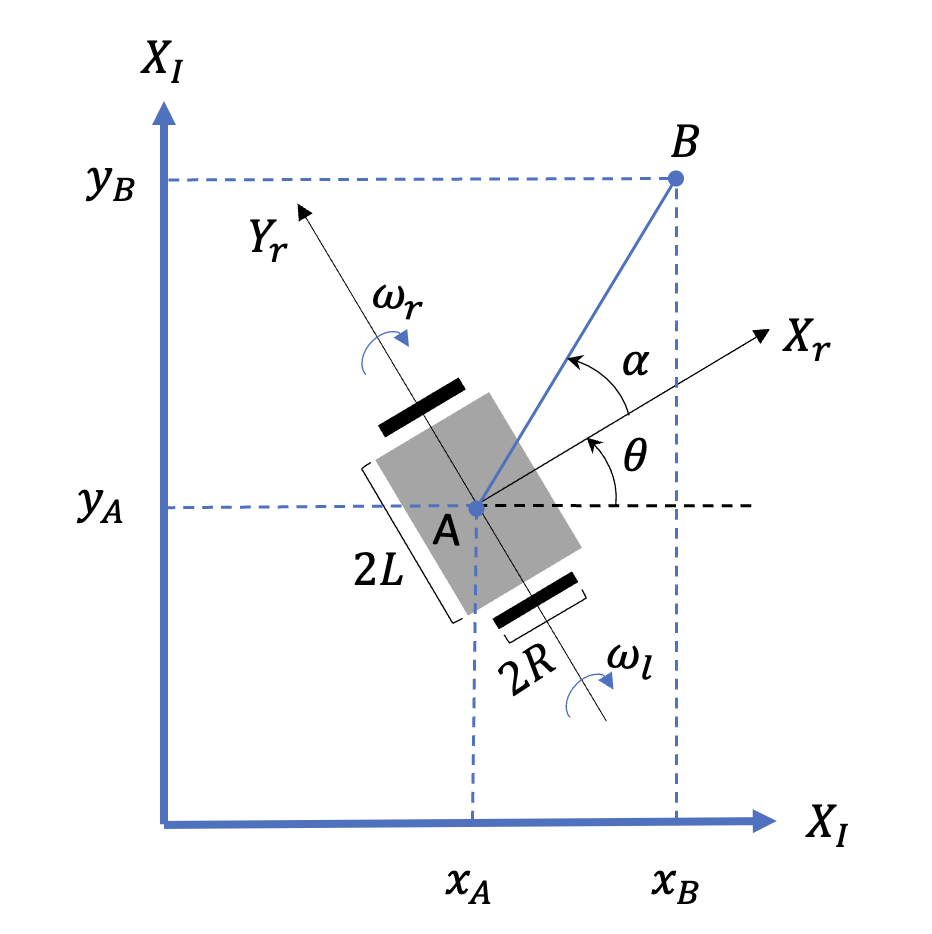
\includegraphics[width=\textwidth]{Diagrams/DDMR.pdf}
                \caption{Differential Drive Mobile Robot}
                \label{fig:DDMR}
            \end{subfigure}
            \hfill
            \begin{subfigure}[b]{0.4\textwidth}
                \includegraphics[width=\textwidth]{Diagrams/WIP.pdf}
                \caption{Wheeled Inverted Pendulum}
                \label{fig:WIP}
            \end{subfigure}        
            \caption{Robot subsystems}
            \label{fig:2DOF}
        \end{figure}


        \subsubsection{Differential Drive Mobile Robot}
    Wheeled mobile robots are typically restricted to navigation in the 2D Cartesian plane. For small robots 
    this configuration, motion models are often simplified by discounting the nonlinear dynamics of friction and 
    the inertial forces arising from acceleration in the $X'$ direction are negligible \cite{KinematicWheeled}. 

    The DDMR's nonlinear kinematics are obtained from Fig.\ref{fig:DDMR} describe point $G=(x_g,y_g)$ as the position of 
    the robot in the global frame.
        \begin{equation}
            \begin{bmatrix}
                \dot x_g \\
                \dot y_g \\
                \dot \psi
            \end{bmatrix}
    =
            \begin{bmatrix}
                \cos(\psi) & 0 \\
                \sin(\psi) & 0 \\
                0 & 1
            \end{bmatrix}
            \begin{bmatrix}
    v_g \\
                \omega_g
            \end{bmatrix}
            \label{eq:DDMRGlobal}
        \end{equation}

    Where the angular velocity $\omega_g$ and linear velocity $v_g$ are the control 
    inputs to the system. 

    The motion of the DDMR is bounded by its non-holonomic constraints, 
    preventing lateral movement along the $Y'$ axis. 
    Under the pure rolling assumption, the wheels do not slip, and the robot's kinematics 
    are governed by the wheel radius $r$ and wheelbase $d$. These parameters define 
    the mapping between the left and right wheel velocities, $\omega_L$ and $\omega_R$, 
    and the global velocities $v_g$ and $\omega_g$, by:
        \begin{equation}
            \begin{bmatrix}
    v_g \\
                \omega_g
            \end{bmatrix}
    =
            \begin{bmatrix}
                \frac{r}{2} & \frac{r}{2} \\
                \frac{r}{d} & -\frac{r}{d}
            \end{bmatrix}
            \begin{bmatrix}
                \omega_L \\
                \omega_R
            \end{bmatrix}
            \label{eq:DDMR}
        \end{equation}

        
        \subsection{DC Motor Model}    
    The robot is driven by two DC motors, through planetary gearboxes, as shown in Fig.~\ref{fig:DCMotor}.
    When a voltage $V_a$ is applied, the DC motor generates a torque, $\tau$, 
    proportional to the armature current, $i_a$.
    According to Lenz's law, the back electromotive force (emf), $e_a(t)$, 
    opposes the applied voltage. These relations are given by:
        \begin{subequations}
            \begin{align}
                \tau &= K_t i_a \\
    e_a &= K_e \dot{\phi}_r
            \end{align}
        \end{subequations}
    where $\dot{\phi}_r$ represents the rotor's angular velocity. The torque 
    and back emf constants are denoted as $K_t$ and $K_e$, respectively.
        \begin{figure}[H]
            \centering
                \includegraphics[width=0.75\textwidth]{Diagrams/DcMotorModel.pdf}
            \caption{Gearbox DC Motor Model Diagram}
            \label{fig:DCMotor}
        \end{figure}
    In small motors, since $L_a \ll R_a$, the electrical dynamics can be approximated as:
        \begin{equation}
    i_a (t) = \frac{V_a (t) - K_e \dot{\phi}_r (t)}{R_a}
        \end{equation}

    The rotor torque, $\tau_r$, is transmitted through the gearbox, which 
    reduces the angular velocity of the wheel, $\dot{\phi}_w$, by the gear ratio $n = \frac{N_2}{N_1}$. 
    Assuming the gearbox is lossless the wheel torque, $\tau_w$, is given by:
        \begin{equation}
                \tau_w = n\tau_r
        \end{equation}
    where $N_1$ and $N_2$ are the number of teeth on the input and output gears, respectively.
    The rotor's inertia $J_r$ and the drive train damping, $B_r$ and $B_g$, are also considered negligible.
    By summing the torques of the rotor and gearbox subsystems, the output torque is given as:
        \begin{equation}
            \tau_w = - J_g \ddot{\phi}_w - \dot{\phi}_w \left( \frac{K_t K_e}{R_a} n^2 \right) + \frac{n K_t V_a}{R_a}
            \label{eq:DCMotorTorque}
        \end{equation}
    where $J_g$ represents the gearbox's inertia and $B_g$ its damping coefficient.

        \subsection{Wheeled Inverted Pendulum}
    The wheel inverted pendulum (WIP), is similar to the classic inverted pendulum on a cart. 
    The WIP is composed of 2 rigid bodies, the body and the chassis connected by a revolute joint, 
    at the center of mass of the wheel as shown in Fig.\ref{fig:WIP}. 
    The center of mass of the body, $B=(x_b,z_b)$, 
    is located at a distance $L$ from the wheel's axel, displaced at some pitch angle $\theta$ with 
    the vertical axis $Z$. The body is assumed to be a point mass $M_b$ with a moment of inertia $J_b$ 
    about the axis of rotation. 
        
    The system of equations governing the time evolution of the WIP are well known.
        \cite{frankovsky2017modeling} \cite{ModelingWIPLagrange}.
    This paper uses the 2DOF state space model as obtained by \cite{Velazquez2016VelocityAM} since it describes 
    the hardware of a similar configuration to the TWSB designed in this project. 
    Incorporating the torque produced by each actuator, eq(\ref{eq:DCMotorTorque}),
    and reiterating the no-slip condition 
        \begin{equation}
            \phi_w = \frac{x}{r}
        \end{equation}
    the model is re-expressed in the notation of this report as 
        \begin{equation}
            \begin{bmatrix}
            \dot{x} \\
            \ddot{x} \\
            \dot{\theta} \\
            \ddot{\theta} 
            \end{bmatrix} =
            \begin{bmatrix}
            0 & 0 & 0 & 0\\
            0 & \frac{2n^2 K_t K_e }{r^2 R_a W_1 } & \frac{-M_b^2 L^2 g}{W_1 \left(J_b +M_b L^2 \right)} & 0\\
            0 & 0 & 0 & 1\\
            0 & \frac{2n^2 K_t K_e }{r^2 R_a W_2 } & \frac{-M_b^2 L^2 g}{W_2 \left(\left(J_b +M_b L^2 \right)+W_1 g\right)} & 0
            \end{bmatrix}
            \begin{bmatrix}
    x\\
            \dot{x} \\
            \theta \\
            \dot{\theta} 
            \end{bmatrix} +
            \begin{bmatrix}
            0\\
            -2n\frac{K_t }{W_1 R_a r}\\
            0\\
            -2n\;\frac{K_t }{W_2 R_a r}
            \end{bmatrix}
    V_a
        \label{eq:2DOF}
        \end{equation}

    with 
        \[
    W_1 = 2\left(\frac{-n^2 J_g + J_w }{r^2 } - M_w \right) - M_b + \frac{M_b^2 L^2 }{J_b + M_b L^2 }
        \]
        \[
    W_2 = W_1 \left(\frac{J_b }{M_b L} + L\right)
        \]

    Where $M_w$ is the mass of the wheel, $J_w$ is the moment of inertia of the wheel.
    \pagebreak{}

    \section{System Design}
        The robot must be designed to approximate the wheel-inverted pendulum system, many authors 
        construct demonstrators supporting a mass with a rectangular structure built out of lead screws. 
        This allows for experimentation with the system's center of mass and is simple to construct. 
        A proof of concept system was developed in this manner, however, the exposed electronics were 
        susceptible to damage during tuning of the balance and navigation algorithms.

        As such the TWSB body is 3D printed out of PLA plastic in 3 parts for minimal assembly.
        The battery pack is quickly swappable and both it and the electronics sub-assembly 
        are soft-mounted in a roll cage-like housing for protection against impacts. 
        The wheels are protected by wheel arches which serve to minimize risk of damage to the motor shaft on wheel impacts. 
        Wiring harnesses are routed through channels to minimize snagging and disconnection from vibrations.
        
        \begin{figure}[H]
            \includegraphics[width=\textwidth]{DesingImgs/bBot Drawing v3.pdf}
            \caption{CAD Drawing of the TWSB system dimensions in mm}
            \label{fig:CAD}
        \end{figure}

        Two brushed DC motors are powered by an H-Bridge IC, DRV7783. 
        The STM32F411RE Microcontroller Unit (MCU) is used to control the 
        motors and monitor the 6 6-axis inertial Measurement Unit (IMU) over I2C. It communicates with the 
        Raspberry Pi 5 over UART via a custom ASCII protocol discussed in section 3.1. 
        The system is powered by a 12V nominal Li-ion Battery pack. A USB-C CC-CV charger is used for quick 
        and accessible recharging, critical for mobile robotics applications. 
        Battery voltage is monitored by the MCU and the pack is protected by a BMS.
        A simple circuit adapted from \cite{chu2008designing} is used to safely load share between the battery pack and the charger.

        \subsection{Software Architecture}
        The modern standard for robotics software is the Robot Operating System 2 (ROS2) \cite{Macenski2022RobotOS}. 
        It is composed of several highly configurable applications that are designed to be managed in a distributed system.
        Distributed systems are beneficial in robotics development as they functionally decouple the software components, 
        enabling robust failure recovery and ease of integrating new features. This concept is useful for this project as 
        the core control and vision systems are developed in parallel. The controls, logs, and error recovery systems mandate 
        high availability compared to user interfaces such as the remote control web app. 
        Whilst this is a powerful tool, it is deemed too complex to learn to meet the project deadline.
        Nevertheless, some core concepts are used such as sharing state by message passing between components, 
        and dynamic parameter configuration to improve testing and data collection. The ZeroMQ middleware is used for 
        timestamped signal stream communication between the computational nodes. 
       
        The software, written in C++, is managed by Systemd as a service. 
        Self-diagnosis routines are used for resource monitoring and auto-recovery. 
        Programs operate on runtime parameters through Remote Procedure Calls (RPC) 
        interface using a GET-SET pattern. This reduces the 
        compile flash debug iteration time. A GStreamer pipeline sets up a video 
        server accessible over LAN. OpenCV is used for optimized image processing.
             
        The firmware is implemented in C using register definitions from the 
        libopencm3 project \cite{BeginningSTM32} as an exercise in low-level programming. 
        No dynamic memory allocation is used.
        The resultant binary is 19KB with 892B of RAM used.
              
        The data-acquisition system obtains a timestamped sample of the 
        telemetry values transmitted by the MCU through a serial link, which implements the
        RPC interface over uart at 230400 baud, 
        it executes commands and publishes telemetry packets at 100Hz.
        Parsing the UART IO buffer can result in non-uniformly sampled data as it
        is constrained by the OS scheduler, thus an event-driven system is used to 
        minimize CPU overhead.
               \subsubsection{Parameters }
        The system parameters are given in Table \ref(tab:SysParams). 
        The mass of the sub-components is obtained by weighing,
        and estimates of the 3D printed parts' mass are given by the slicer software. 
        The CAD files are used in MATLAB's Multibody Simulink environment, which 
        computes the center of mass and the moments of inertia can subsequently be estimated.
        The Motor parameters are estimated through the system identification experiments discussed in section 3.2.
                    
        \begin{table} [H]
            \centering
            \begin{tabular}{|c|c|c|c|}
                \hline
                Parameter & Value & Units & Description \\
                \hline
                $M_b$ & 0.8 & kg & Mass of the body \\
                $L$ & 0.08135 & m & Height of COM above wheel axel \\
                $J_b$ & 0.0071& kgm$^2$ & Moment of inertia of the body \\
                $r$ & 0.04 & m & Radius of the wheel \\
                $M_w$ & 0.09 & kg & Mass of wheel assembly \\
                $J_w$ & 0.000072 & kgm$^2$ & Moment of inertia of the wheel \\
                $d$ & 0.132 & m & Wheel base \\
                $R_a$ & 1.5 & $\Omega$ & Resistance of the motor \\
                $K_t$ & 0.24 & Nm/A & Torque constant of the motor \\
                $K_e$ & 0.18 & V/rad/s & Back EMF constant of the motor \\
                $n$ & 20 & - & Gear ratio \\
                $J_g$ & 0.0003 & kgm$^2$ & Moment of inertia of the gearbox \\
                \hline
            \end{tabular}
            \caption{System Parameters}
            \label{tab:SysParams}
        \end{table}

        \subsection{System Identification}
        A set of experiments are conducted to evaluate the transfer function of the motors.

        \begin{table}[H]
            \centering
                \begin{tabular}{|r|c|c|c|c|c|c|}
                    \hline 
                    Gear Ratio & Rated Torque & Rated Speed  & Rated Current & Stall Current & Stall Torque \\
                    \hline
                     1:20  & 0.39 Nm & 600 rpm & 500 mA & 2 A & 0.15 Nm/Kg \\
                    \hline
                \end{tabular}
                \caption{Manufacturer Provided Motor Parameters}
        \end{table}

        A telemetry and analysis software system developed in Python. It is used as 
        test bench  setup shown in Fig.\ref{fig:SysIDSetUp}, a series of reference 
        ramp, step, sine, and chirp inputs are applied to each motor.

        The test suite contains a time-series signal generator, with preview and playback functionality.
        The system logs and messages are displayed in a terminal window, and the user can fully configure 
        each node's runtime parameters remotely over a network connection, utilizing the RPC ASCII protocol.
        A line plotter is configured by JSON to display any number of signals the robot may produce.
        This architecture allows for repeatability in obtaining robot data, something 
        is is a challenge in mobile robotics.
        
        \begin{figure}[H]
            \centering
            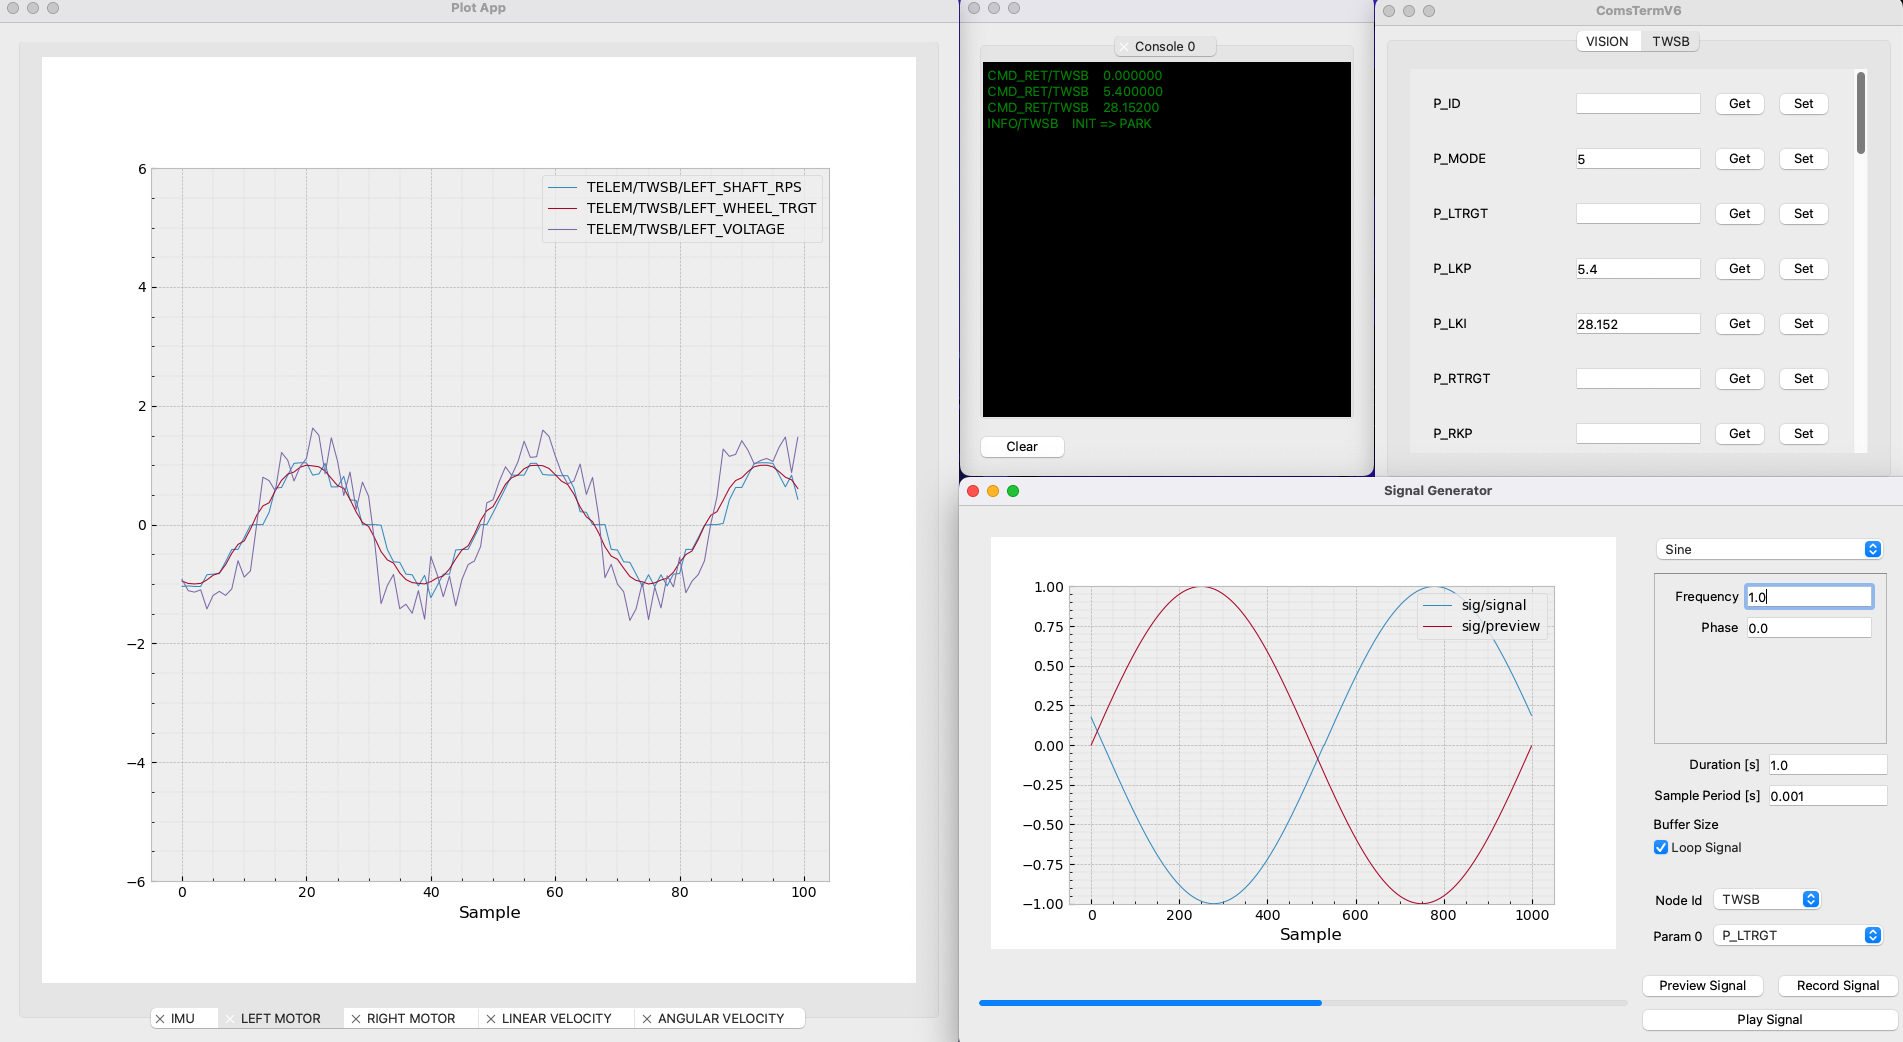
\includegraphics[width=0.9\textwidth]{SysIDMotorSetUp.png}
            \caption{System Identification Testbench Setup}
            \label{fig:SysIDSetUp}
        \end{figure}
      
        This software system is also utilized for heuristic tuning of the control
        and vision systems. The program can visualize control signal streams in soft real-time 
        and provides a useful insight into the effects of the control system on the plant.

        \begin{figure}[H]
            \centering
            \begin{subfigure}[b]{0.45\textwidth}
            \includegraphics[width=\textwidth]{Graphs/OpenLoopStep.pdf}
            \caption{Open Loop Step Response}
            \label{fig:openstep}
            \end{subfigure}
            \hfill
            \begin{subfigure}[b]{0.45\textwidth}
            \includegraphics[width=\textwidth]{Graphs/1HzSine.pdf}
            \caption{Open Loop Sine Response}
            \label{fig:opensine}
            \end{subfigure}
            \caption{Open Loop no Load Speed Voltage Experiments}
            \label{fig:openloop}
        \end{figure}

        From these experiments, it is clear that the motor has significant deadzones, 
        and the input-output relationship is nonlinear at low armature voltages. 
        The maximum no-load speed within the manufacturer's operating range is found to be 8 rotations per second.
        To increase control authority, the motors are powered by 12V, with the armature voltage modulated by 
        the duty cycle of the PWM signal. The DRV7783 Integrates current sensing and over-current protection,
        used to limit the current to the motors to 1.5A.
              
        For stationary balancing of the TWSB robot
        the actuators are required to operate mostly in a sinusoidal fashion, 
        similar to Fig.\ref{fig:opensine}, to regulate the pitch angle of the body.
        Considering this a closed-loop controller is developed in section 5.1 to regulate the motor speed,
        and maintain the device in its operating region. 
       
           \section{State Estimation}
        Information about the TWSB system may be obtained from 2 kinds of sources; 
        mathematical models models as in eq(\ref{eq:2DOF}) which can describe the time evolution of the chosen system variables, 
        and sensors that convert energy arising from a physical property into information. Both of these sources 
        are approximations of the true state. The process of combining multiple sources of information is termed sensor fusion.
        This section evaluates the available methods employed using \textit{proprioceptive} sensors.
           \subsection{Sensors Overview}
        For the TWSB system in eq(\ref{eq:2DOF}) its state variables $\theta$ and $\dot x_b$ can be measured through the onboard IMU 
        and the wheel encoders respectively. 
                   
        The motors incorporate a low-cost 12 pulses per revolution (PPR) incremental encoder on the rotor shaft. 
        Further resolution is easily obtained by using the MCU's quadrature 
        peripheral to increment, or decrement, a counter based on the phase transitions.
        Considering the gearbox ratio $n=20$, an effective resolution of 960 PPR is attained.
        The rotational speed of the wheel is computed by sampling the change in the pulse counts
        over a sample period $\Delta t$. Thus the error in the velocity estimate, 
        is inversely proportional sample period, resulting in larger errors at low speeds.
        Yet, it is observed that more significant sources of error arise from the mechanical backlash in the gearbox.
        The sample time is set to 2 ms, and a low-pass filter is given by the infinite recursive relation as
        \begin{equation}
            y_k = \alpha x_k + (1-\alpha)y_{k-1}
            \label{eq:lpf}
        \end{equation}
        exponentially attenuates sudden deviations in the velocity estimate by selecting $\alpha = 0.95$.
       
        Using this velocity estimate in the model of the DDMR from eq(\ref{eq:DDMRGlobal}) to obtain the
        position of the robot in the cartesian plane as ($x_g,y_g$) is known as odometry.
        There are various sources of errors in 
        this process, arising from assembly imperfections and conditions in 
        the environment which may break the constraints assumed in the kinematics of the DDMR.
                   
        These conditions become significant in the case of the TWSB system as crashes, or bumps, result in large 
        and unbounded error accumulation. In the case of crashes, the robot is subsequently stationary 
        and its state is reset. However, in the case of bumps, where the robot can recover, corrective 
        action is required to mitigate this. Assuming a sufficiently accurate wheel encoder, a simple method is 
        implemented based on \cite{Gyrodometry}, only correcting 
        the odometry when such events are detected.  
        This leads to the decision that other forms of systematic odometry errors have to be 
        either disregarded in the short term or corrected by landmark methods by $exteroceptive$ sensors. 
       
        The IMU is a 6-axis MEMS sensor \cite{ComplimentaryKalman} which measures the local linear acceleration 
        and angular velocity.
        The 3D acceleration, $\vec{a}$, is used to obtain an 
        estimate of the pitch angle as $\hat{\theta} = \mathrm{atan2}\left(-a_x ,a_z \right)$
       
        The variance of this $\hat{\theta}$ is small when the system is at rest but grows larger when subject to vibration from the motors
        as shown by the experiment in Fig.\ref{fig:accelNoise} where the TWSB is placed horizontally at rest and motor control commands are issued. 
        \begin{figure}[H]
            \centering
            \begin{subfigure}[b]{0.5\textwidth}

                \includegraphics[width=\textwidth]{Graphs/accelNoiseReadings.pdf}
                \caption{Accelerometer is sensitive to motor vibrations}
                \label{fig:accelRaw}
                
            \end{subfigure}
            \hfill
            \begin{subfigure}[b]{0.45\textwidth}
                \includegraphics[width=\textwidth]{Graphs/noisyPitchEst.pdf}
                \caption{Wide Variance on pitch estimate at rest}
                \label{fig:pitchNoise}
            \end{subfigure}
            \caption{Accelerometer Noise}   
            \label{fig:accelNoise}
        \end{figure}

        From \ref{fig:pitchNoise} it can be seen that the IMU is not mounted perfectly orthogonal to the body frame. 
        \begin{table}[H]
            \centering
            \begin{tabular}{c c c} 
                \toprule
                $a_{x_0}$ & $a_{y_0}$ & $a_{z_0}$ \\
                \midrule
                0.036453 & -0.0021066 & 0.133658 \\
                \bottomrule

            \end{tabular}
            \caption{Accelerometer Mounting Offset (m/s$^{2}$)}
            \label{tab:accelOffset}
        \end{table}
        This systematic error is removed by utilizing calibrated values in Table \ref{tab:accelOffset}.
        \subsection{Kalman Filter}
        The Kalman Filter (KF) and its variants  are widely used in robotics to fuse 
        complementary sources of information \cite{Thrun2005ProbabilisticRobotics} \cite{perez2023quadcopter} \cite{Moore2014AGE}.
        Even though the state transition model of the TWSB robot is non-linear \cite{ooi2003balancing} 
        developed self-balancing platforms capable of restricting oscillations about the 
        operating point to $±1$ degree. This is one order of magnitude than the worst-case linearization pitch limit of $±10$ degrees.
        Beyond this, the small angle approximation is no longer valid, and the system is not locally linear. As such it is determined 
        that if the controller is able to regulate the pitch to within this range, then the optimum linear estimator known as the Kalman Filter is suitable.

        The Kalman Filter is a 2-stage recursive estimator which uses the system model to predict the state of the system,
        and then corrects this prediction using the measurements from the sensors. The notion of a prediction and correction 
        stems from Bayesian statistics, where signals are modeled as random variables with a probability distribution.
        The Kalman Filter is applicable to linear systems, and as such the random variables are assumed to be normally distributed. 
        Considering a linear stochastic system of the form:

        \begin{equation}
            x_t = A_t x_{t-1} + B_t u_t + \epsilon_t
        \end{equation}

        where $\epsilon_t$ is a noise term with zero mean and covariance $Q_t$. The Kalman Filter is concerned with 
        updating its posterior belief in the true state of \textit{bel}$(x_t)$ with some weighted sum of the 
        information from the prior belief \textit{$\bar{\text{bel}}(x_t)$}, the current measurement $z_t$, and the evolution of 
        the model of the system through the control action $u_t$.

        At each time step $t$, the TWSB system obtains new measurements from its sensors, which are related to the state space by:

        \begin{equation}
            z_t = C_t x_t + \delta_t
        \end{equation}

        where $\delta_t$ is a noise term with zero mean and covariance $R_t$.  
        Often noise variables of this kind are denoted as part of the $N(0, R_t)$ group of random variables.
        The matrix $C_t$ maps the measurements to the state space as a linear transformation.

        Before the measurement can be used, the Kalman Filter must first obtain an estimate of the state given the 
        prior belief and the control action. This is termed the prediction stage, where the current mean, given the prior mean, 
        is predicted through applying the current control action to the system model. This prediction increases the uncertainty of the belief through the 
        process noise, which is a random variable given as $N(0, Q_t)$. This process noise is assumed to be independent from the measurement noise.
        The prediction step is given by the equations:

        \begin{equation}
            \mu_{t|t-1} = A_t \mu_{t-1|t-1} + B_t u_t
        \end{equation}
        \begin{equation}
            P_{t|t-1} = A_t P_{t-1|t-1} A_t^T + Q_t
        \end{equation}

        By the linearity of Gaussian distributions, incorporating the measurement will reduce the uncertainty in the posterior belief. 
        This is done through the Kalman Gain matrix as:

        \begin{equation}
            K_t = P_{t|t-1} C_t^T (C_t P_{t|t-1} C_t^T + R_t)^{-1}
        \end{equation}
        \begin{equation}
            \mu_{t|t} = \mu_{t|t-1} + K_t (z_t - C_t \mu_{t|t-1})
        \end{equation}
        \begin{equation}
            P_{t|t} = (I - K_t C_t) P_{t|t-1}
        \end{equation}

    
        The state transition model used by the KF can be chosen to model the TWSB system eq(\ref{eq:2DOF}) as a step towards 
        full state feedback, or solely based the dynamics of the IMU.
            
        The MPU6050 6-Axis IMU can be used to  estimate the pitch through the 
        gyroscope measurement $\vec\omega_{gyro}$, which due to its mass spring construction, even if miniutrazizred, suffers from a drift noise term. 

        \begin{equation}
            \vec\omega_{gyro} = \omega + b_g + n_g
        \end{equation}

        and the accelerometer measurement \ensuremath{\vec{\alpha}_{accel}} is from as 
        
        \begin{equation}
            \vec{\alpha}_{accel} = \alpha - g + b_a + n_a
        \end{equation}
        Where the external acceleration arising form linear motion is given as $\alpha$, accelerometers bias by $b_a$ and noise by $n_a$. 

        A Kalman Estimator is developed to fuse the gyroscope and accelerometer measurements, using the model of the IMU obtained similar to \cite{ComplimentaryKalman}.
        This is implemented on the microcontroler at 1Khz.  

        \begin{figure}[H]
            \centering
            \includegraphics[width=0.8\textwidth]{Graphs/SensorFusion.pdf}
            \caption{Sensor Fusion of accelerometer and gyroscope}
            \label{fig:SensorFusion}
        \end{figure}
             
        Fig.\ref{fig:SensorFusion} shows that the Kalman Filter's produces a smooth estimate of the pitch angle
        under conditions of the experiment in Fig.\ref{fig:accelNoise}. 
        \pagebreak{}

    \section{Control System}
        Autonomy in mobile robotics is commonly a hierarchical problem composed of high-level path planning, 
        or task allocation, and low-level control of the actuators.  
        Successful implementations must design solutions to both of these problems in a complementary manner in order 
        to achieve the desired system behavior, of tracking the planned configurations.
                
        For the TWSB robot, behavior can be described by two main goals, static balancing and navigation.
        These two behaviors are inherently coupled due to the system's underactuated design. Hence, the 
        magnitude of the feedback required for sufficiently fast stabilization leads to significant chatter or oscillations 
        in the control signal.
    
        Gain scheduling is suggested by \cite{refvem2019design}
        as a way to operate the system in these two different modes. A similarly underactuated system is controlled via this 
        method by \cite{wanggain}. Notably, in these cases care must be taken to ensure 
        that discontinuities in the control signal at the point of switching do not cause instability \cite{hespanha2002switching}.
        Determining the switching schedule is a nontrivial problem, often mandating experimental validation-dependent 
        on the systems parameters, \cite{RoboLimbo} utilizes advanced nonlinear strategies to determine these
        boundary conditions.
    
        The tracking performance of reactive control strategies is often bounded by the control effort 
        demanded within the bandwidth of the actuators. Typically in feedback systems, a saturation function 
        is utilized on the reference to enforce safe operation. This discontinuity breaks the linearity of the 
        controller often leading to oscillations, and care must be taken to avoid such limit cycles.
                
        The PID regulator is an attractive choice for many systems, as by nature of negative feedback it does not 
        require an explicit model of the plant to operate. The process variable is typically a direct measurement 
        obtained by a sensor, and the control law $u_k$ is computed reactively to an error signal at each timestamp $k$.
        Oftentimes, intuition about the signal's physical units is sufficient to tune the feedback gains adequately. 
        However, performance validation in the model-free case must be evaluated at runtime, this may prove to be 
        challenging or destructive in cases of unstable or safety-critical systems. 
            
        Heuristic methods such as Ziegler-Nichols formulate approaches to black-box tuning of a plant by observing the system 
        performance under sustained instability and designers experimentally tune such algorithms.
        For example, from the input-output data of the selected actuators obtained in Fig.\ref{fig:openloop}, 
        it can be seen that a large integral action is needed to overcome the steady-state error.
        This is a common issue in low-cost DC motors, where the static friction of the gearbox presents 
        a nonlinearity which is most notable at low control authority and difficult to model. 
        
        Model-based control allows the designer to validate the performance of the system in simulation. 
        Often frequency domain tools are used to analyze the plant in an open loop. From this, a control law is designed around 
        the controllable state variables with physical information on the behavior of the system.
        Given a model of the system, designers also can formulate constraints, 
        and obtain an optimal control signal which meets these. For example, by minimizing the control effort in a cost function
        the challenges associated with choosing a saturation safety function can be mitigated.
        
        Parameter uncertainty is a common issue in controlling mobile robotics, and approximations of these often lead to 
        discrepancies between the mathematical optimal solutions found in simulation \cite{eide2011lqg} 
        and in real world performance \cite{tran2023fuzzy}. The difficulty with purely model-based approaches is
        the need for a high-fidelity model and access to low-uncertainty measurements of the state variables.
        
        A model of a TWSB robot, incorporating the non-idealities of low-cost DC motors is proposed by \cite{yamamoto2008nxtway}.
        It is used together with a simulation study of a WIP platform as a reference solution for the TWSB problem.
    
        Another approach is to use actuators with more favorable characteristics for the task at hand, such as stepper motors.
        The static balancing problem aims to control $\theta$ and regulate the linear displacement. The coupling of the 
        pitch angle to the rate of change in linear position requires active control, resulting in oscillations in both these state variables. 
        Stepper motors draw a nominal current, thus maintaining high torque at low speeds, eliminating the need for gearboxes and the 
        backlash associated with them. 
                
        The field of adaptive control proposes dealing with system uncertainties by designing controllers that may 
        learn over time. Online trial-and-error data and statistical techniques like regression-based transfer
        function estimation from input-output data are used to develop physics-informed models taken under statistical 
        distributions of belief \cite{benosman2018model}.         
                    
        In a similar vein, \cite{williams2016aggressive} embeds a neural network as an online function approximator to learn 
        predictions of the dynamics of the system. This prediction is then used as part of a trajectory planner in race-line optimization. 
        Some modern microcontrollers have sufficient computational power requirements needed for Model Predictive Control (MPC) and 
        effective implementations of convex optimizers \cite{nguyen2024tinympc} have been used in small mobile robots \cite{giernacki2017crazyflie}.
                
        An attractive aspect of predictive approaches to control is that they lend themselves naturally to 
        planning long horizons. These methods use numerical simulation techniques to evolve the system over time 
        and estimate the distribution of state probabilities through sampling of control actions. 
        The optimal control sequence is then chosen from these samples using a cost function.
                    
        The autonomous behavior of the TWSB robot explored in this paper is that of the path 
        following in an unknown environment, where no prior map is available. As such the 
        the control system has three goals, namely disturbance rejection of the pitch angle; 
        this is required such that the system is robust to the environment, minimizing 
        the linear displacement when stationary and tracking a trajectory obtained by a 
        high-level planner discussed in section 6. 
    
        A simple PID controller operating on the pitch error is tested in a simscape multibody; 
        a physics-based simulation where the control law is an applied force to a prismatic joint. 
        This force is coupled through the revolute joint to the pitch angle as described by \ref{eq:2DOF}.
        This manages to stabilize the pitch angle yet the $x$ position drifts over time as this 
        state variable is not controlled.
        More complete control laws are discussed in the following sections.
        \subsubsection{Controler requirements}

        The TWSB achieves balance by controlling the oscillations of the pitch angle about the 
        vertical axis. The linear system of equations in eq.(\ref{eq:2DOF}) is applicable 
        only when the pitch angle is small, this is taken to be $\theta < ±10$ degrees. 

        The advanced non-linear control methods discussed above are beyond the scope of this project. 
        Whilst their performance guarantees under real-world conditions are attractive, it is often simpler 
        to implement complex behaviors in the high-level planner.
        In the sequence, the low-level controls are developed to meet these requirements:
        \begin{enumerate}
            \item The pitch angle must be regulated to $±1$ degree.
            \item The robot must be able to safely recover from disturbances due to external forces and the environment.
            \item The robot must be able to track a reference velocity, with minimum overshoot.
        \end{enumerate}

        \subsection{Cascade PID}
                
        In the planer case shown in Fig.\ref{fig:WIP} the trajectory of the center of mass is parametrized by 
        the pitch angle $\theta$ and the linear velocity $v_b$. 
            
        A cascaded PID controller is used to control the pitch angle and the linear velocity. 
        Control of the position $(x_g,y_g)$ is left to a higher-level planner.  
        If the inner loop dynamics are much faster than the outer loop, 
        then the inner loop can be approximated as a disturbance \cite{Robust2DofPID}.

        Again, simscape multibody is used to verify the feasibility of this kind of controller Fig.\ref{fig:SimPID}.

        \begin{figure}[H]
            \centering
            \includegraphics[width=0.7\textwidth]{Graphs/Simulation Cascade PID.pdf}
            \caption{Simscape Multibody Simulation of PID Cascade Controller regulating the linear velocity of the TWSB}
            \label{fig:SimPID}
        \end{figure}

        Through the Ziegler-Nichols method, the PID gains for each DC Motors speed control loop 
        are obtained. This process however may cause damage to the motors 
        during the sustained oscillations at the critical gain. 
        To determine the maximum operating frequency of the outer loop, 
        the inner motor speed loop is closed at 500Hz. Then the system is observed under chirp inputs to the motor, and from 
        these responses, the error of the pitch angle is subsequently regulated by a PID controller operating at 100Hz.
       
        This results in a stable system in 1DOF space. To minimize chatter in the pitch angle control signal, the outermost 
        loop controlling the body velocity is closed at 20Hz.
        The final cascaded closed loop PID controller is shown in Fig.\ref{fig:Cascade} with the gains in Table \ref{tab:PIDGains}. 
        This control system is able to adjust its target balancing point in such a manner as to come to an equilibrium, overcoming small 
        errors in the construction of the robot which might result in a center of mass that is not directly above the wheel axel. 
        Without the outermost loop controller, the TWSB is sensitive to this error and the offset must be tuned experimentally.
       

        \begin{figure}[H]
            \includegraphics[width=\textwidth]{Diagrams/cascade.pdf}
            \caption{Cascaded PID Controller}
            \label{fig:Cascade}
        \end{figure}

        \begin{table}[H]
            \centering
            \begin{tabular}{|r|r|r|r|c|c|c|c}
                \hline
                & \multicolumn{5}{c|}{Process Variable}  \\
                \hline
                Parameter & $v_b$ & $\theta$  & $\omega_L$ & $\omega_R$ & $\dot{\psi_b}$ \\
                \hline      
                $K_p$ & 3.5 & 0.19 & 2.4 & 2.9 & 0.7 \\
                $K_i$ & 0.8 & 5.6 & 24.8 & 24.8 & 0 \\
                $K_d$ & 0 & 0.003 & 0 & 0  &  0 \\
                \hline
            \end{tabular}
            \caption{Control system PID Gains}
            \label{tab:PIDGains}
        \end{table}
      
        \pagebreak{}
        \section{Navigation System}

        The TWSB robot is tasked with navigating around a track, marked by a line assumed to be of significant contrast to to its 
        surrounding environment. The performance of the navigation system can be characterized by the cross-track error and the lap time, 
        with the former being a critical failure mode, if the position diverges significantly from the track in a non-recoverable manner.

        \begin{figure}[H]
            \centering
            \includegraphics[width=0.6\textwidth]{TestTrack.pdf}
            \caption{Test Track, (1) Chicane, (2) Hairpin, (3) Wall Proximity, (4) Straight, (5) Shallow Curvature, (6) Apex}
            \label{fig:TestTrack}
        \end{figure}

        The reference track tests common navigation tasks and challenges highlighted in Fig.\ref{fig:TestTrack}. 
        Here the environment is nonideal as the floor has various textures, marks, and colors.
        Lighting conditions are also nonuniform and the track is physically bounded by walls on all sides, enforcing hard accuracy constraints. 
        When teleoperated using the camera feed, it is challenging to avoid crashes. A human operator with 
        a full view of the environment can navigate the robot around the track, at moderate speeds the line is often lost 
        from the camera view. This mandates a corrective action using information about the robot's global pose, 
        which is not available to the TWSB. This track is therefore a suitability-challenging test for autonomous mobile navigation.
                   
        Map building is a popular approach for mobile navigation in a closed loop as it allows for a large 
        context of the environment to be considered. Closed maps can be built iteratively, by exploration 
        and subsequent loop closure. In this case, guarantees can also be made, 
        such as static obstacle avoidance and path selection by optimization functions \cite{Macenski_2020}. 
        This is referred to as global navigation and often requires advanced localization sensors 
        and algorithms to triangulate the robot's pose within the global environment.
               
        In this report, however, no global map data is available and the robot must navigate 
        the track using only the information obtained from the camera sensor. This is commonly known as local navigation
        and is fundamental to autonomous behavior where it is often impractical to obtain and maintain such a map. Without a map, 
        however, the robot must infer its pose relative to the track, and in cases where the track is not visible, the robot is lost. 
        Robust autonomy must be able to handle cases where the robot is lost, and safely search for the track or remain stationary. 
       
        Path following is commonly implemented with a lateral and a longitudinal controller. This follows from the 
        inputs and non holonomic constraints of the DDMR system in eq(\ref{eq:DDMRGlobal}).
        The longitudinal controller regulates the linear velocity of the robot where, in the simplest form, the reference speed 
        is set to a constant value, and the lateral controller keeps the robot heading aligned with the track. 
        This method is suitable for simple tracks and low speeds.
               
        In contrast, trajectory tracking is a method that generates some optimum path from the sensed environment and subsequently follows this path.
        This two stage process is falls under planning and is useful in cases where the lap time is more important than the cross-track error.
        In racing, the robot has to perform at the limits of its handling capabilities \cite{wischnewski2022indy}. Hence a method 
        for automatic safety is required, a common method extends planning by predicting the robot's position over some horizon,
        a velocity profile can be then obtained whilst maintaining the robot within certain bounds, often the profile is 
        designed in such a manner to stop the robot at the end of its horizon \cite{williams2016aggressive}. These kinds of model predictive controllers 
        have been demonstrated to have impressive performance but are complex methods that require a high-fidelity model of the robot within its environment. 
        The time constraints of this project preclude the exploration of data-driven 
        or learning methods employed to build such a model of the TWSB robot. As such a series of reactive controllers are used within different 
        racing-line algorithms based on curvature of the track ahead as baseline methods.
                   
        Many local navigation methods rely on obtaining a geometric representation of the track ahead, effectively building a local map.
        Commonly a path can be represented as a piece-wise arc or a form of cubic spline, from which parameters such as curvature, $\kappa$, 
        can be obtained. Simpler methods of path following by monocular camera have been applied to the TWSB robot, these do not measure the 
        geometry of the track, but rather use the image data to classify a set of features and use these in a rule-based algorithm to follow the 
        track, \cite{visionlinetwsb} \cite{ismail2009vision} \cite{nntwsbvision}.
        These methods are found to limit the track to shallow curvature or low speeds as they only utilize a small 
        a subset of the information available from the camera sensor. 
       
        In this paper, a method is developed that obtains a set of track waypoints from a grayscale monocular camera. 
        Whilst these do not predict the future poses of the robot, the nature of the 
        monocular camera sensor's information allows for a dynamic velocity component to be added to path following.

        \subsection{Camera Sensor}
        Geometric information about the track can be observed from a camera sensor mounted on the TWSB robot.
        This obtains a discreet 2D projection of the environment in the form of a matrix of pixels, each of which encodes 
        its value as an 8-bit unsigned integer. Considering such an image, it is nontrivial to
        obtain a map of the track concerning the robot, as the data is highly encoded in a large measurement space. 
        Perceptual sensors of this form differ from the physical sensors found elsewhere on the TWSB robot as the quantity measured; 
        light intensity, is not directly usable as a state variable, except in simple autonomous behavior like photo-taxis \cite{hasslacher1995living}. 

        The question of what quantifies useful information in an image is a long-standing problem,  \cite{siegwart2011introduction} classifies 
        perception as the process of condensing the detailed information contained within each image, or sequence of images, 
        into features that are useful to track for the task at hand.
        In the case of monocular mobile navigation, the notion of feature models is a key concept in active perception \cite{Activeperception}.
        These models are used to infer $\textit{percepts}$, which are then used to make decisions in controlling the robot's pose within its environment 
                \cite{hutchinson1996tutorial}. 

        The field of computer vision is concerned with the extraction of these percepts from the image data. 
        Classical computer vision algorithms are used to extract spatial information about the sensed environment over the visible 
        horizon. Common features are reasoned by geometry, \cite{lee2009geometric} such as edges, corners, lines, and blobs of texture. 
        These are typically processed using a series of 2D convolutional filters, or kernels, which for large images is
        computationally expensive and often requires the use of a GPU to parallelize the operations. In these cases, the
        advances in parallel computing have proliferated the use of neural networks in computer vision, which apply a 
        series of latent filters to the image data. These are trained on large datasets of images 
        or online \cite{tai2017virtual} \cite{lee2013line} \cite{kober2013reinforcement}, and aim to simply the process of feature extraction. 
                
        The TWSB is equipped with a Raspberry Pi Camera Module V3, which is a rolling shutter camera. Images are obtained 
        in grayscale directly from the Y plane of the camera driver at 640x480 resolution to improve encoding speed and 
        minimize wireless transmission bandwidth.

        \subsubsection{Calibration}
        Cameras are optical devices and are subject to lens and pixel distortion. Modern cameras are assumed to have square pixels, 
        but still require some calibration to undistort the barrel effect of the lens. 
        The camera is mounted on the TWSB robot at a height of 18cm with an angle of 15 degrees to the floor plane.
        This perspective results in rectangles in the environment being projected into trapezoids.  This makes it difficult to 
        obtain distances between different features identified in the image \cite{tuohy2010distance}
        A top-down, orthographic view of the floor plane is desired, where there is a linear function mapping pixel sizes 
        to real-world distances. A chessboard pattern of known dimensions is placed on the floor plane in front of the camera, 
        this encompasses the entire field of view. From the position of the chessboard corners in the image, 
        a homography matrix is obtained which maps the image coordinates to the real-world coordinates \cite{bradski2008learning},
        resulting in the corrected perspective transform shown in Fig.\ref{fig:perspective}. 
        This method assumes the pitch angle, and thus its field of view of the camera to be constant, it it diverges too much the 
        mapping needs to be re-calibrated which is computationally expensive on the Raspberry Pi.
        \begin{figure}[H]
            \centering
            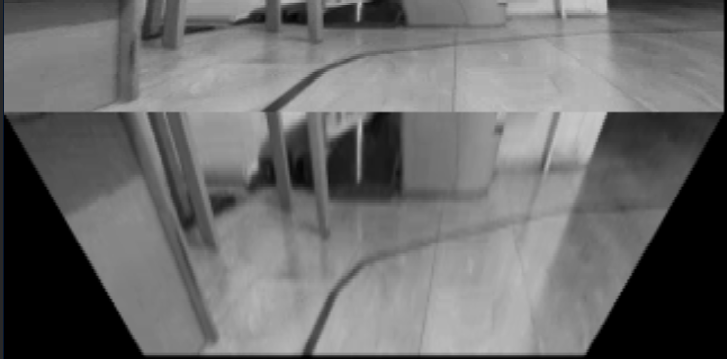
\includegraphics[width=0.6\textwidth]{visionpipeline/perspective.png}
            \caption{Perspective Correction}
            \label{fig:perspective}
        \end{figure}

        \pagebreak{}
        \subsection{Track Detection}
        The robot must be able to obtain an estimate of where the track line is, relative to its forward direction.
        In nonideal environments, significant noise is present in the image data, 
        and simple edge thresholding methods are not sufficient. This noise can lead to large errors
        in the estimated position of the track. The information in the image needs to be condensed into a set of features
        that describe the track. Summing the pixel values in each column, a distribution of the edges 
        across the image is found. The ideal straight line can be thought of as a single peak in the center of the frame.  
        It can be seen in Fig.\ref{fig:Line Detection and Segmentation} that this method results in peaks of different 
        shapes depending on the curvature of the track, however, the track position in the image plane is readily 
        segmented by the peak's topological prominence, that is the difference between 
        a peak and the local minima around it. 
        \begin{figure}[H]
            \centering
            \begin{subfigure}[b]{0.45\textwidth}
                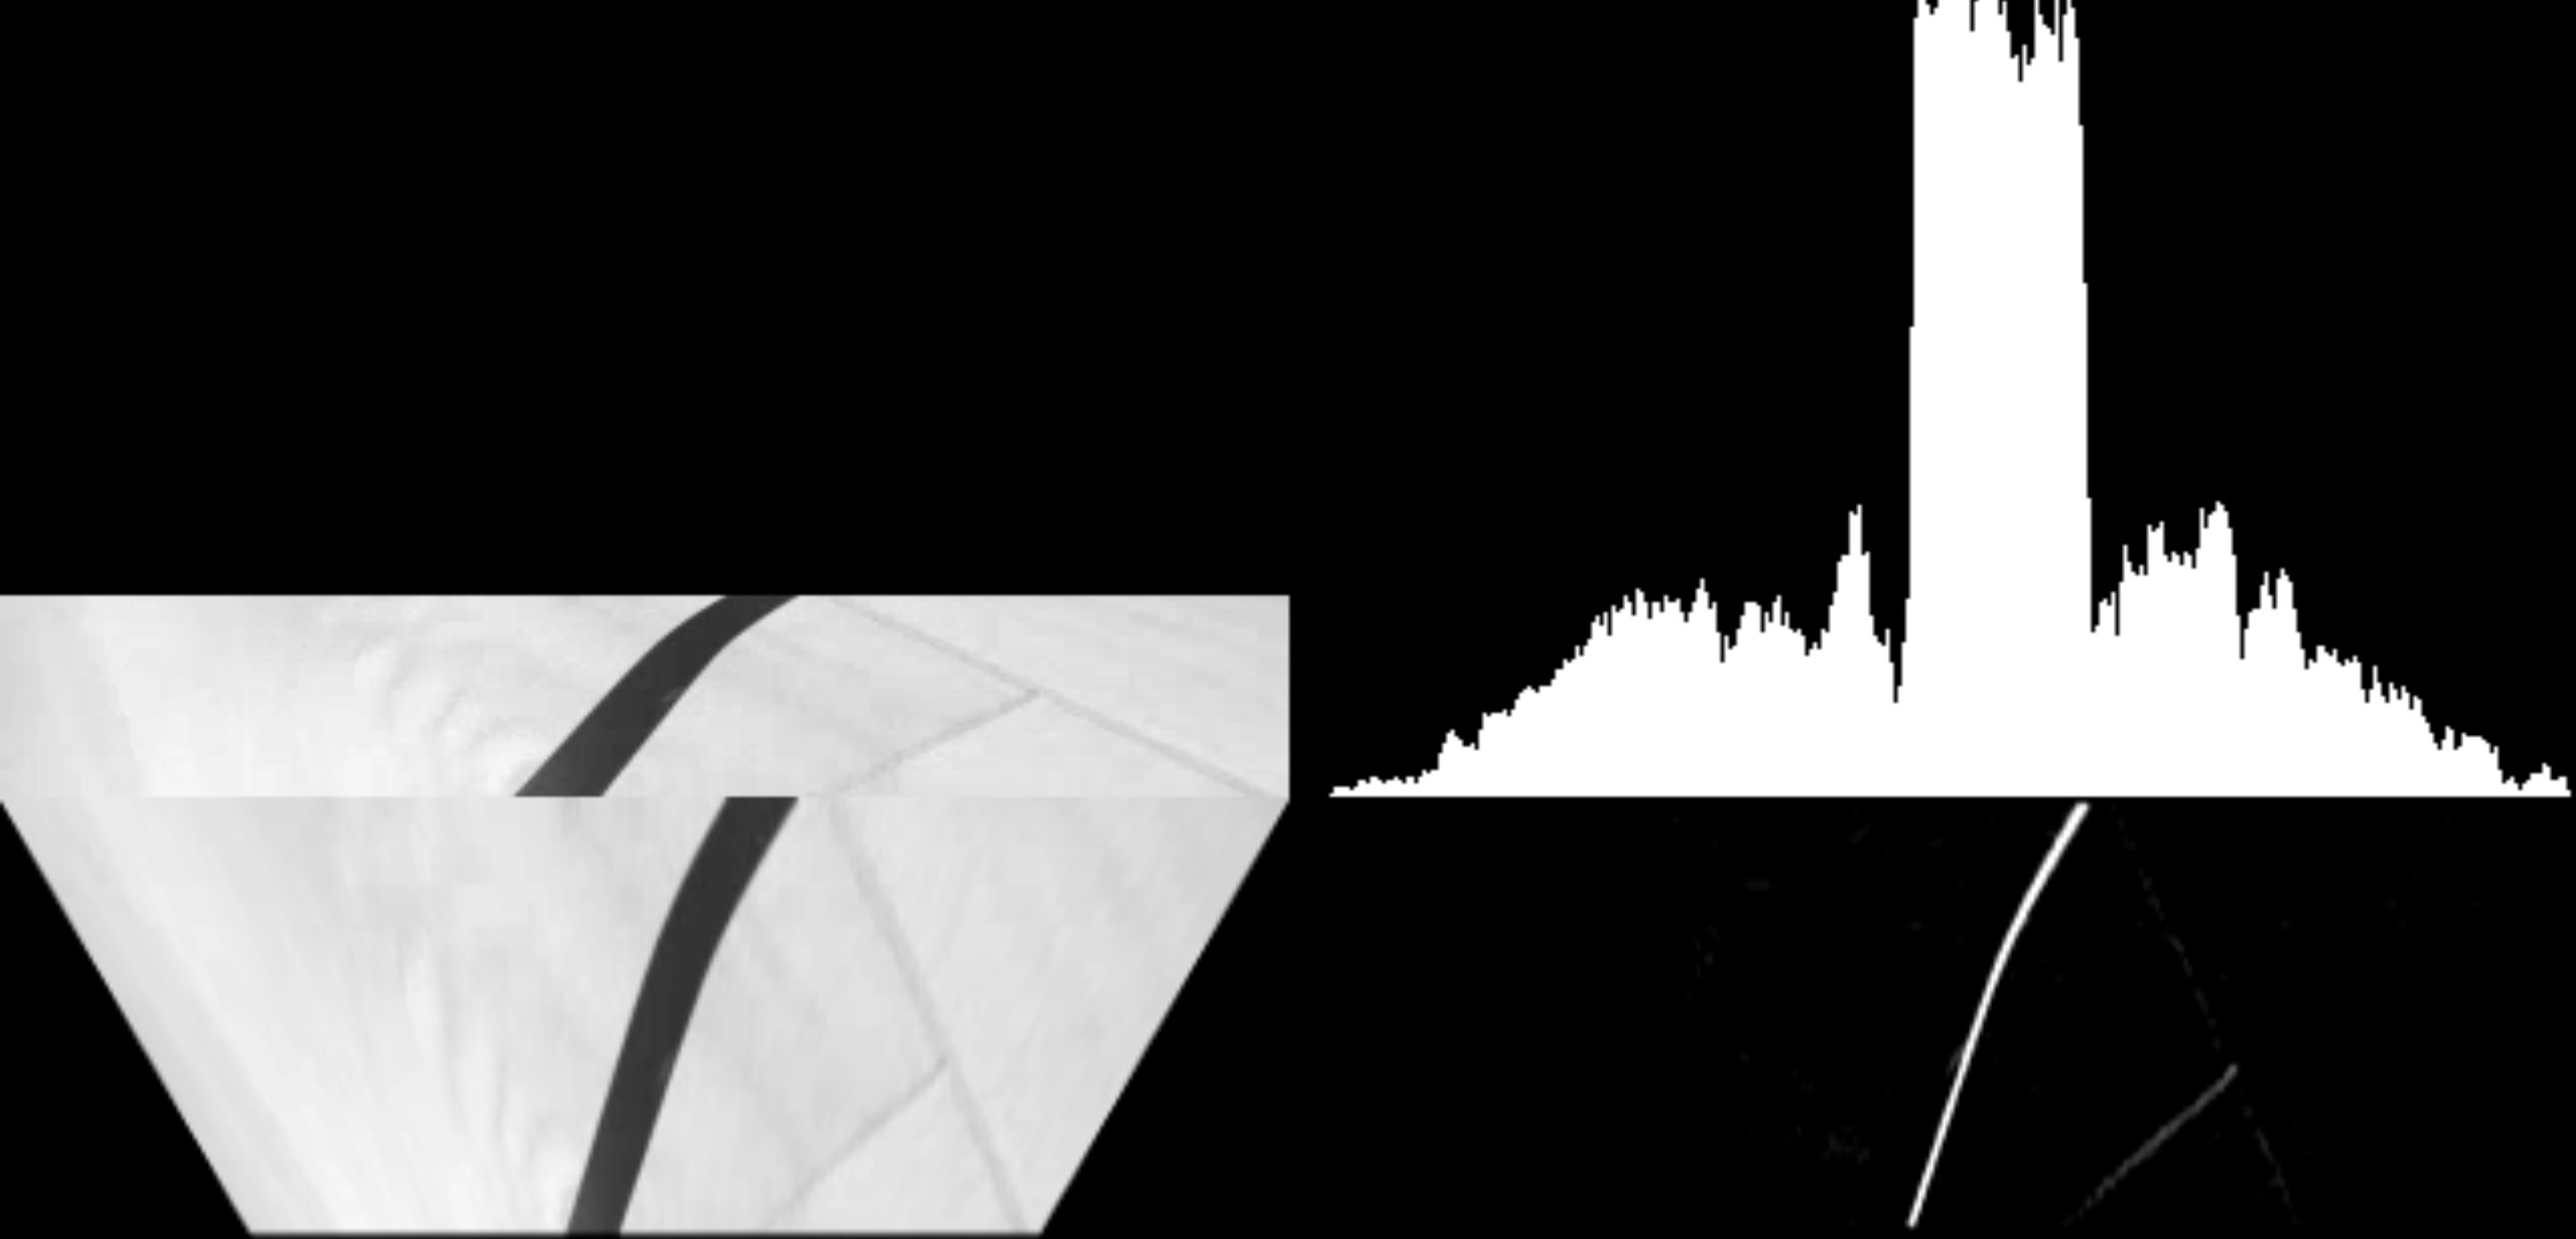
\includegraphics[width=\textwidth]{visionpipeline/vizSmallCurve.png}
                \caption{Low Curvature}
                \label{fig:LineDetection}
            \end{subfigure}
            \hfill
            \begin{subfigure}[b]{0.45\textwidth}
                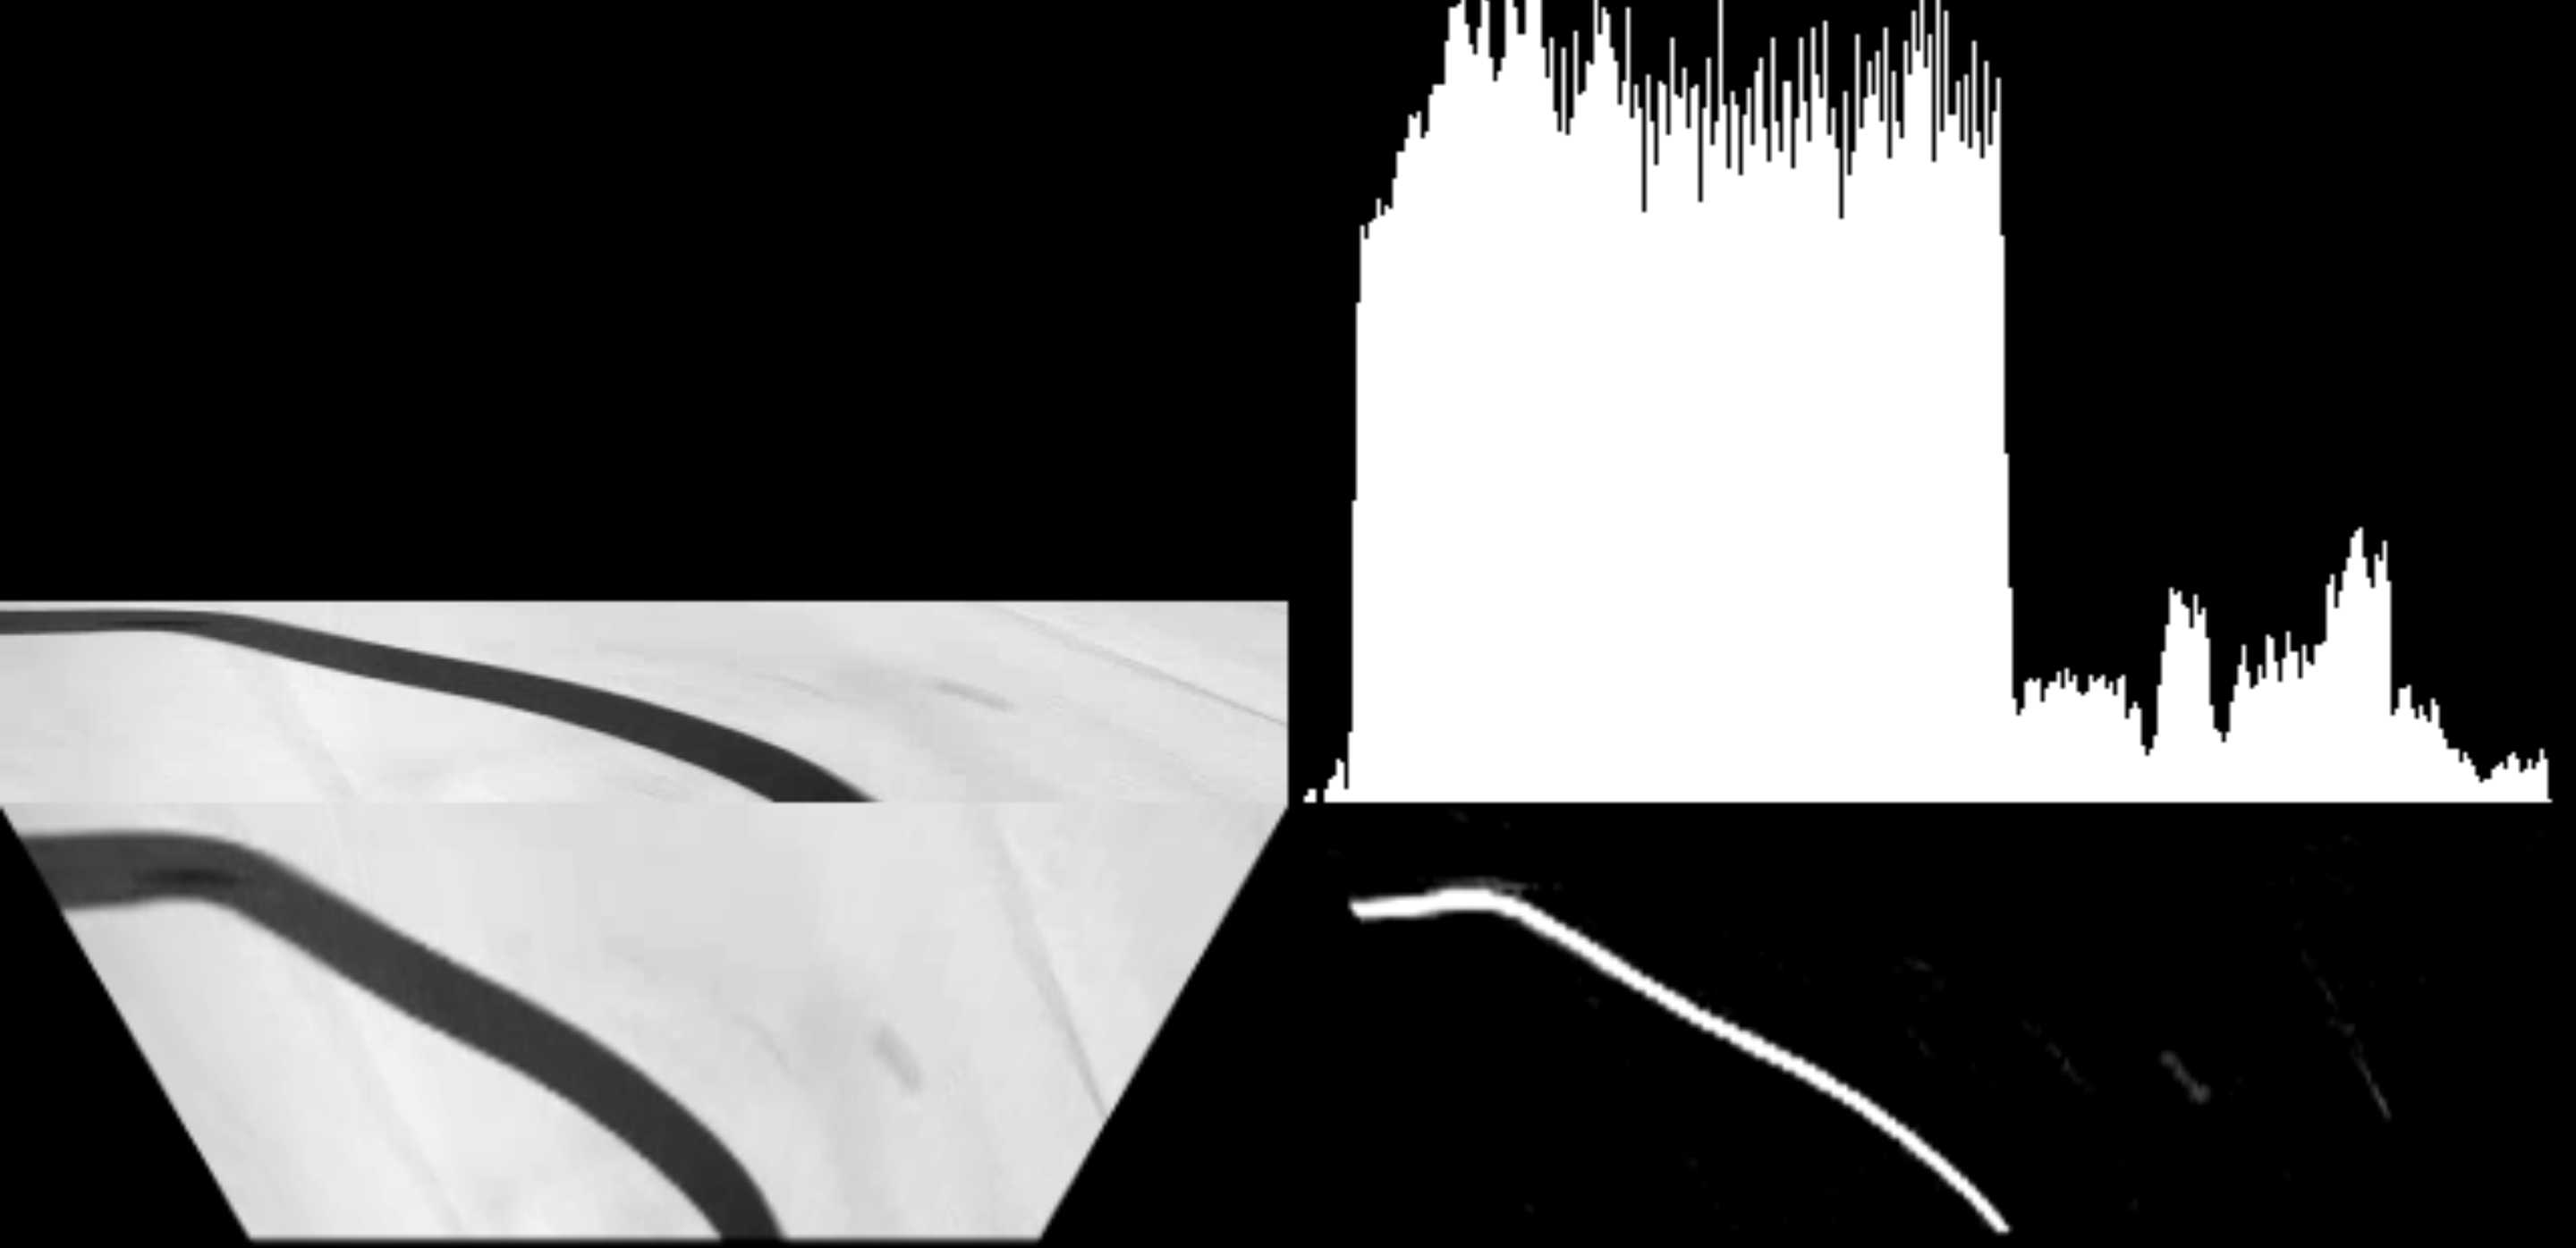
\includegraphics[width=\textwidth]{visionpipeline/vizBigCurve.png}
                \caption{Sharp Curvature}
                \label{fig:Sharp Curvature}
            \end{subfigure}
            \caption{Line Detection and Segmentation}   
            \label{fig:Line Detection and Segmentation}
        \end{figure}
        
        Some challenging cases, where simpler methods may fail, are shown in 
        Fig.\ref{fig:ChallengingEnvironments}. Here it can be seen that these cases have a higher noise floor, 
        that is the the peak is not as prominent. This prominence can be used as an indicator of the confidence that 
        the peak is the true position of the track. 
       

        \begin{figure}[H]
            \centering
            \begin{subfigure}[b]{0.45\textwidth}
                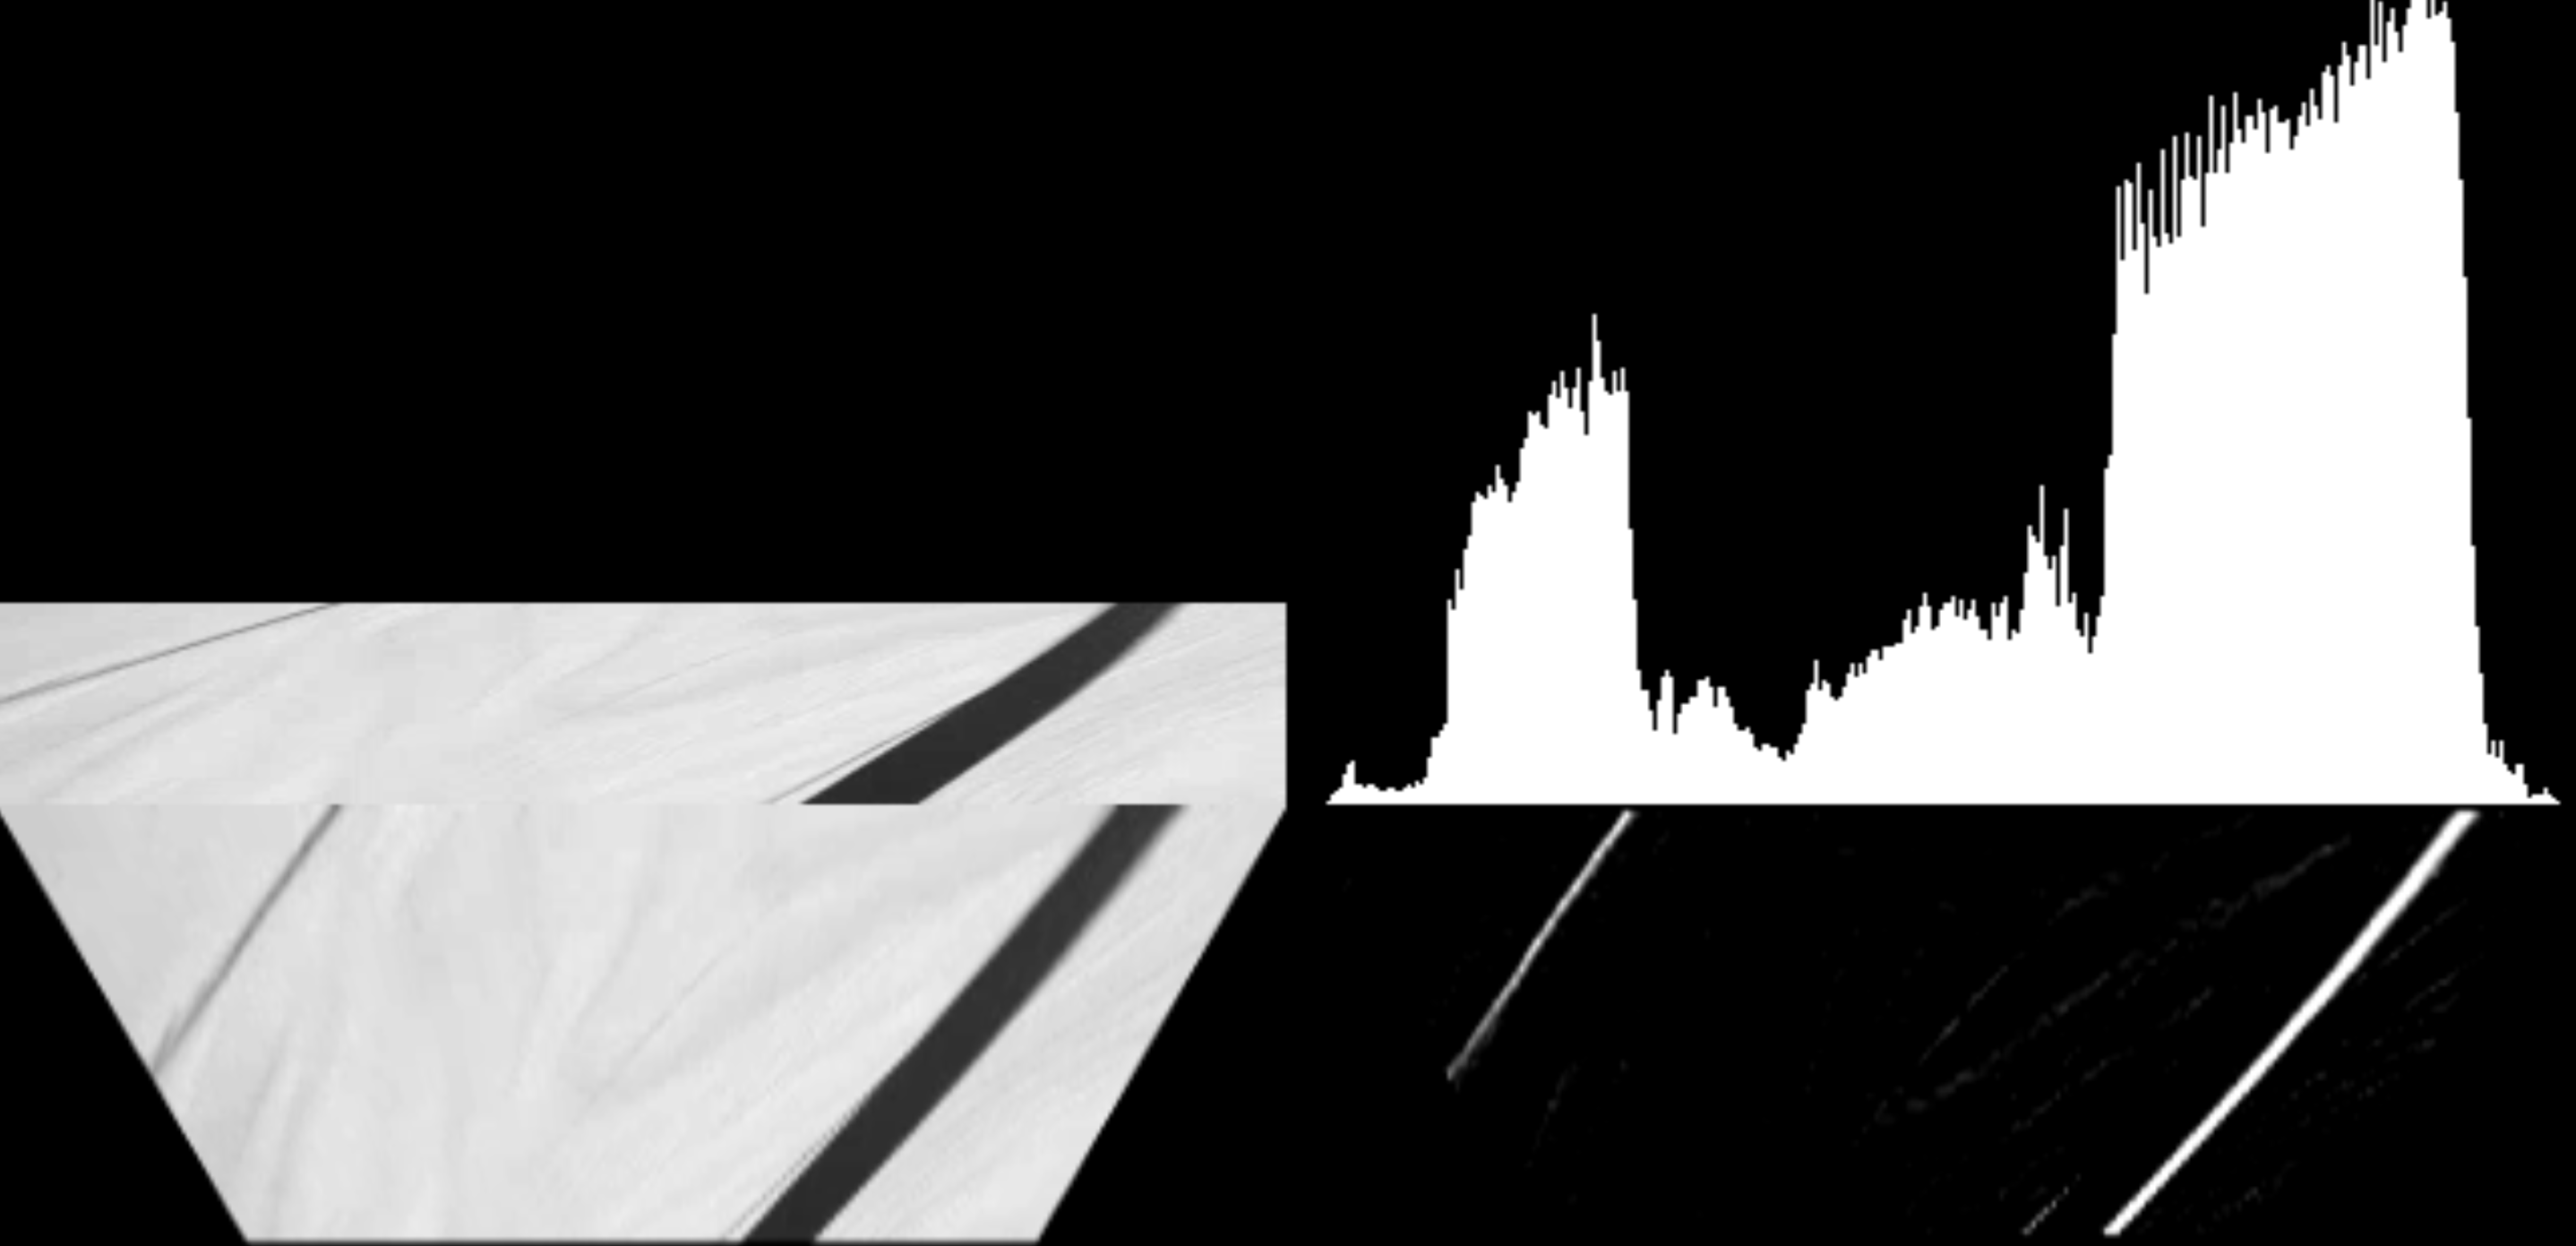
\includegraphics[width=\textwidth]{visionpipeline/vizFalsePos.png}
                \caption{False Positives}
                \label{fig:FalsePositives}
            \end{subfigure}
            \hfill
            \begin{subfigure}[b]{0.45\textwidth}
                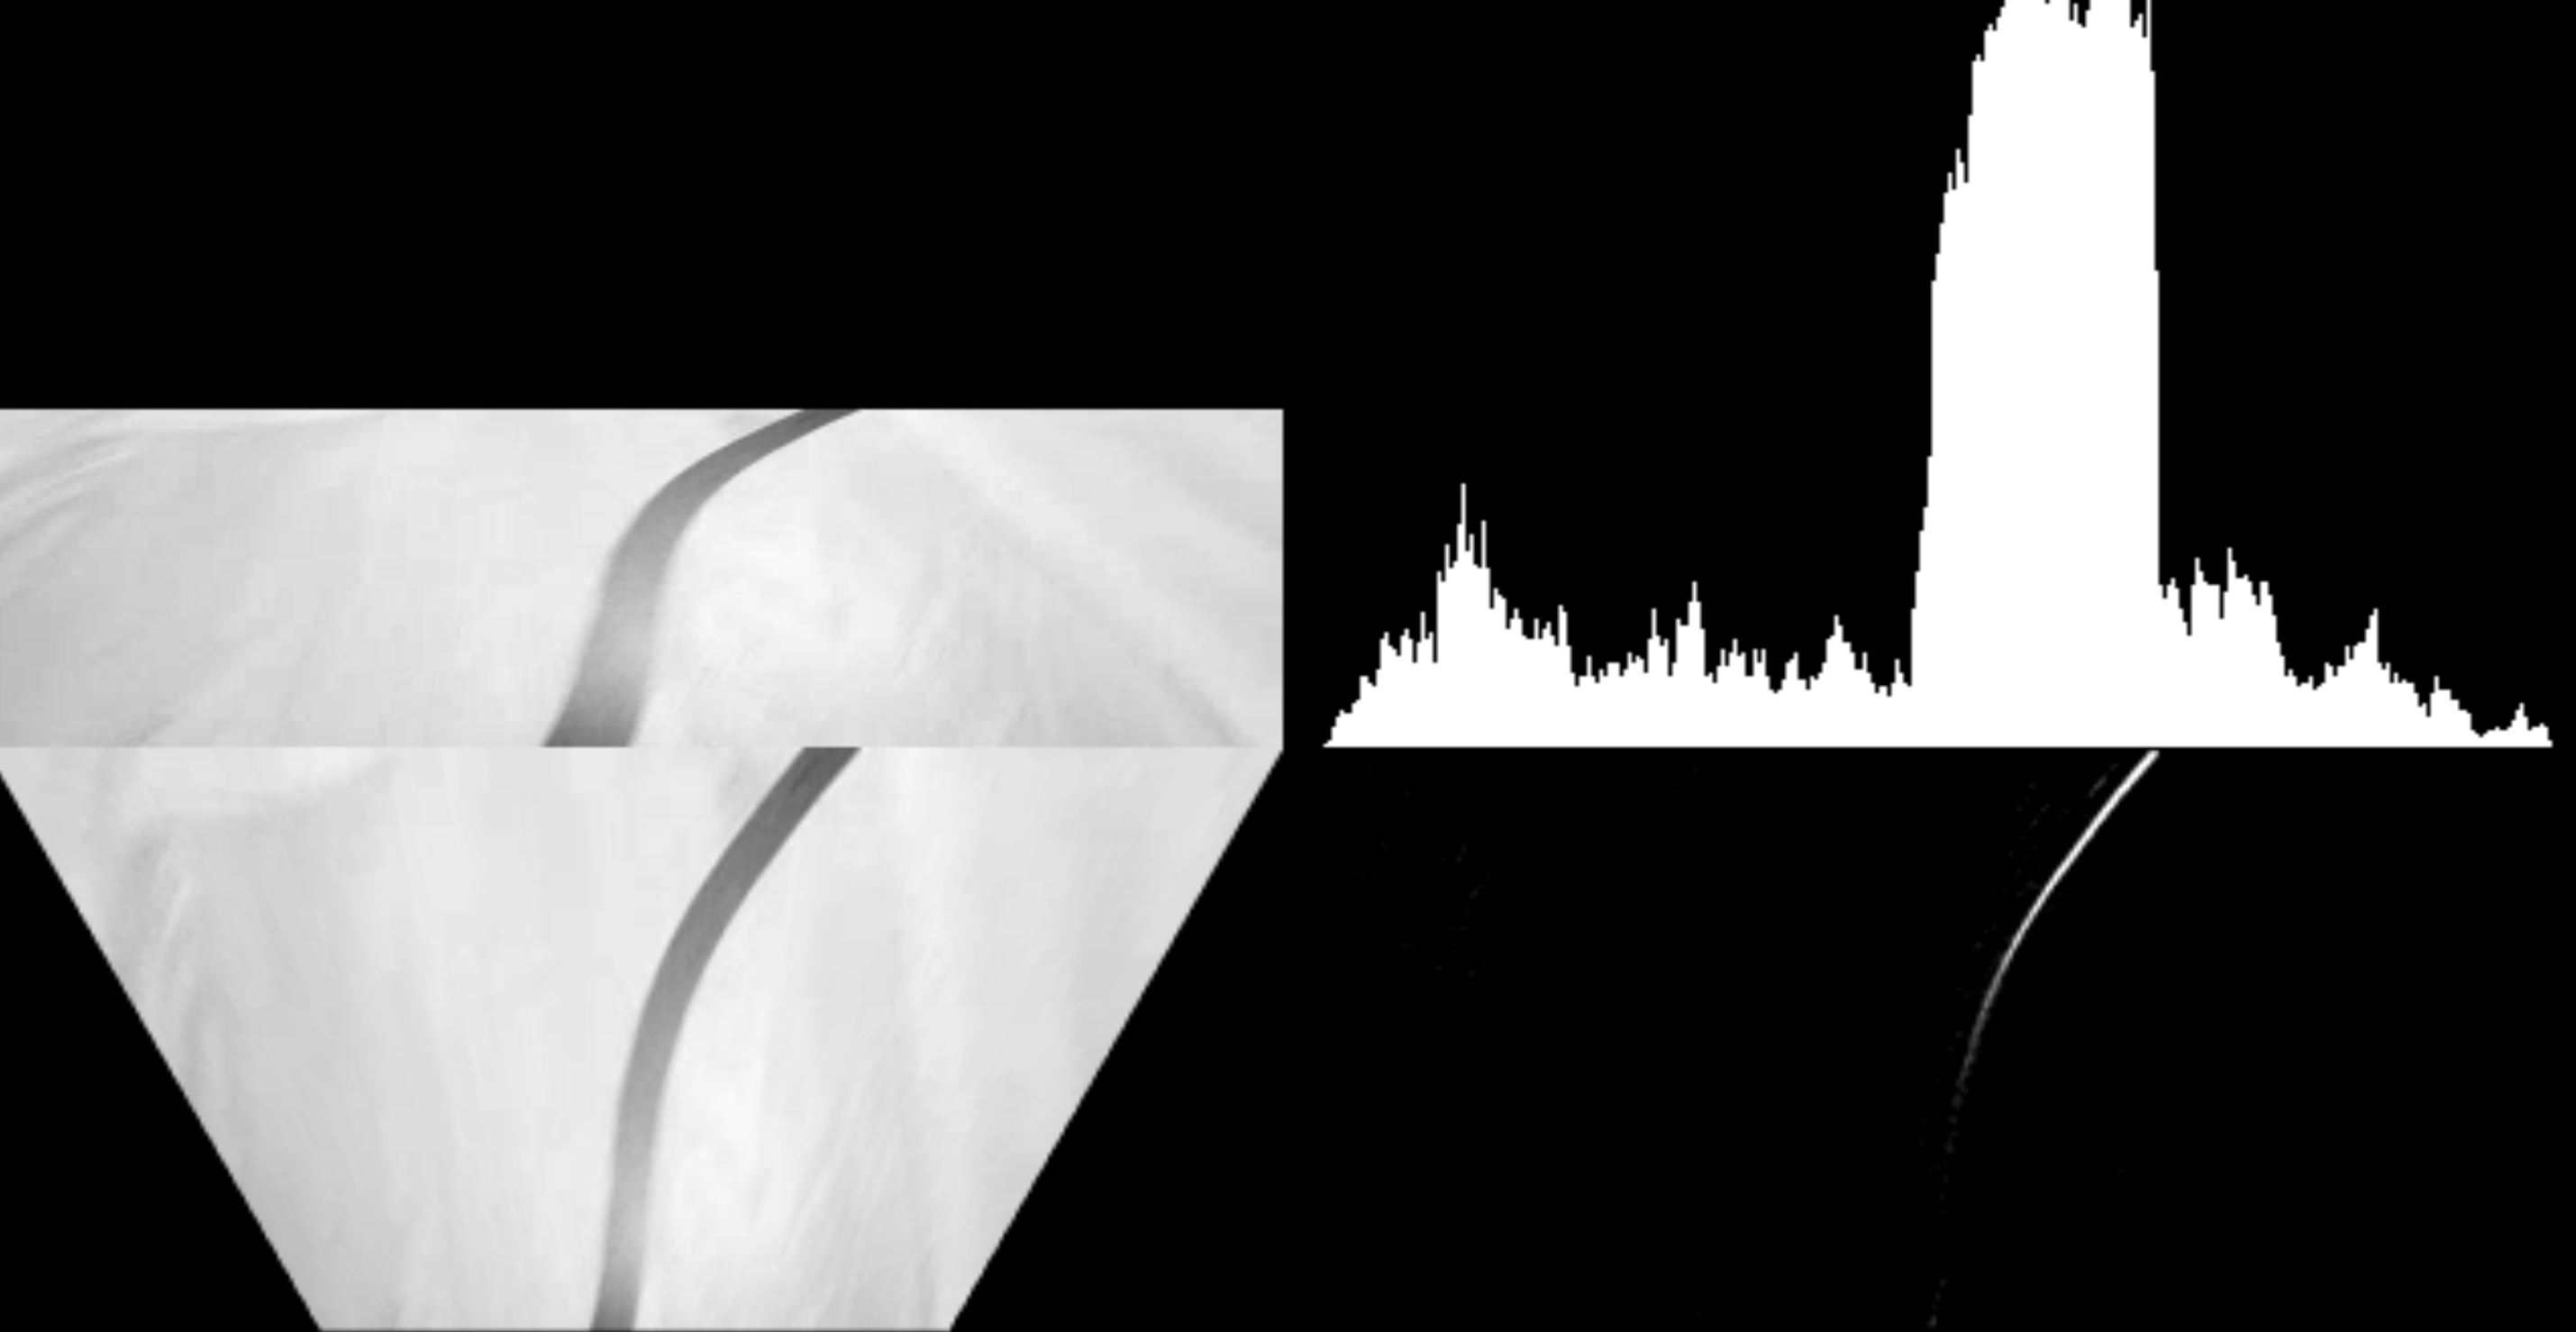
\includegraphics[width=\textwidth]{visionpipeline/vizLightOclusion.png}
                \caption{Reflective Occlusion}
                \label{fig:ReflectOcclusion}
            \end{subfigure}
            \caption{Challenging Environments}
            \label{fig:ChallengingEnvironments}
        \end{figure}


        False positives as shown in Fig.\ref{fig:FalsePositives} are a serious issue with line detection algorithms as 
        they often cause the robot to lose track of the original path in a nonrecoverable manner.
        These are difficult to remove once present in the 1D histogram of the edges, as they form peaks of similar shapes to desired features. 
        This nonunique mapping of data to a set of features is a common issue in robotic perception, as such the control and perception methods 
        must be co-designed to reject these robustly.

        From these images, three sources of noise features are identified: salt and pepper noise, arising mainly through impulses in texture 
        variation of the floor, object boundaries resulting in an edge of a similar shape to the track, and occlusions from reflections 
        or movement blur stemming from the rolling shutter of the camera.

        Pre-filters like the median filter can be used to remove salt and pepper noise, however, this is computationally expensive, taking on average 10ms
        to process a single frame on the selected hardware; resulting in the entire pipelining not running in real-time. 
        The proposed vision pipeline uses morphological operators to modify the shape of the features in the image.
        By eroding and dilating these features, the impulse noise is removed, this lowers the median noise floor, increasing the prominence of the peaks. 
        Assuming that the robot is initially on the track, then the search space for the peak representing the track can be expanded around the last
        known position of the track. Subsequently, the track peak is searched for staring at the bottom of the image, and sliding a window upwards, 
        until a large discontinuity is found. This is done by searching for the largest peak in the histogram, warm starting each section search from the position 
        of the peak found in the section below it, and then checking if the next peak is within a certain distance. In this manner,
        a series of waypoints on the track is obtained, which as shown in Fig.\ref{fig:LineDetection} are robust to the sources of noise discussed. 
        The algorithm processes each frame and obtains a continuous set of waypoints describing the track on average in 0.15ms when running on the Raspberry Pi 5.
        \begin{figure}[H]
              \centering
              \begin{subfigure}[b]{0.32\textwidth}
                 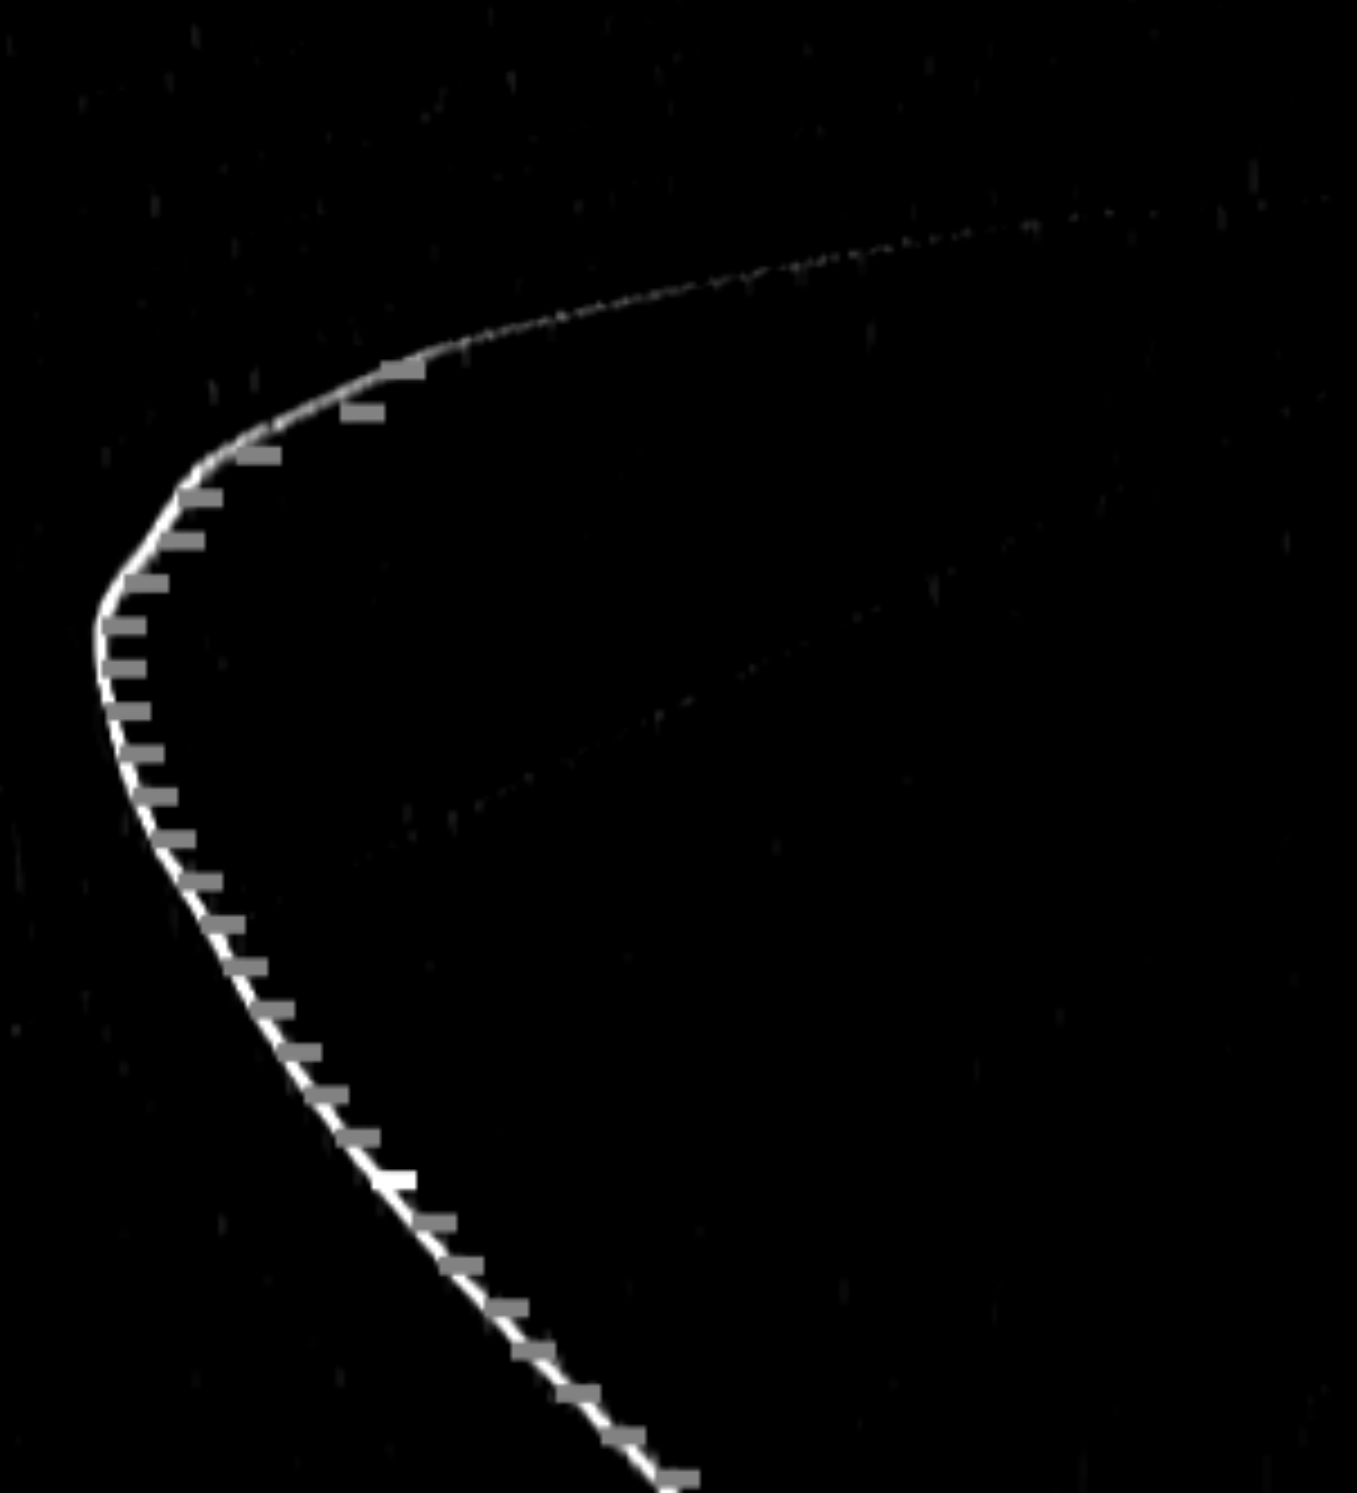
\includegraphics[width=\textwidth,height=0.2\textheight]{visionpipeline/curverightapprach.png}
                 \caption{Right Curve Approach}
                 \label{fig:appoachRight}
              \end{subfigure}
              \hfill 
              \begin{subfigure}[b]{0.32\textwidth}
                 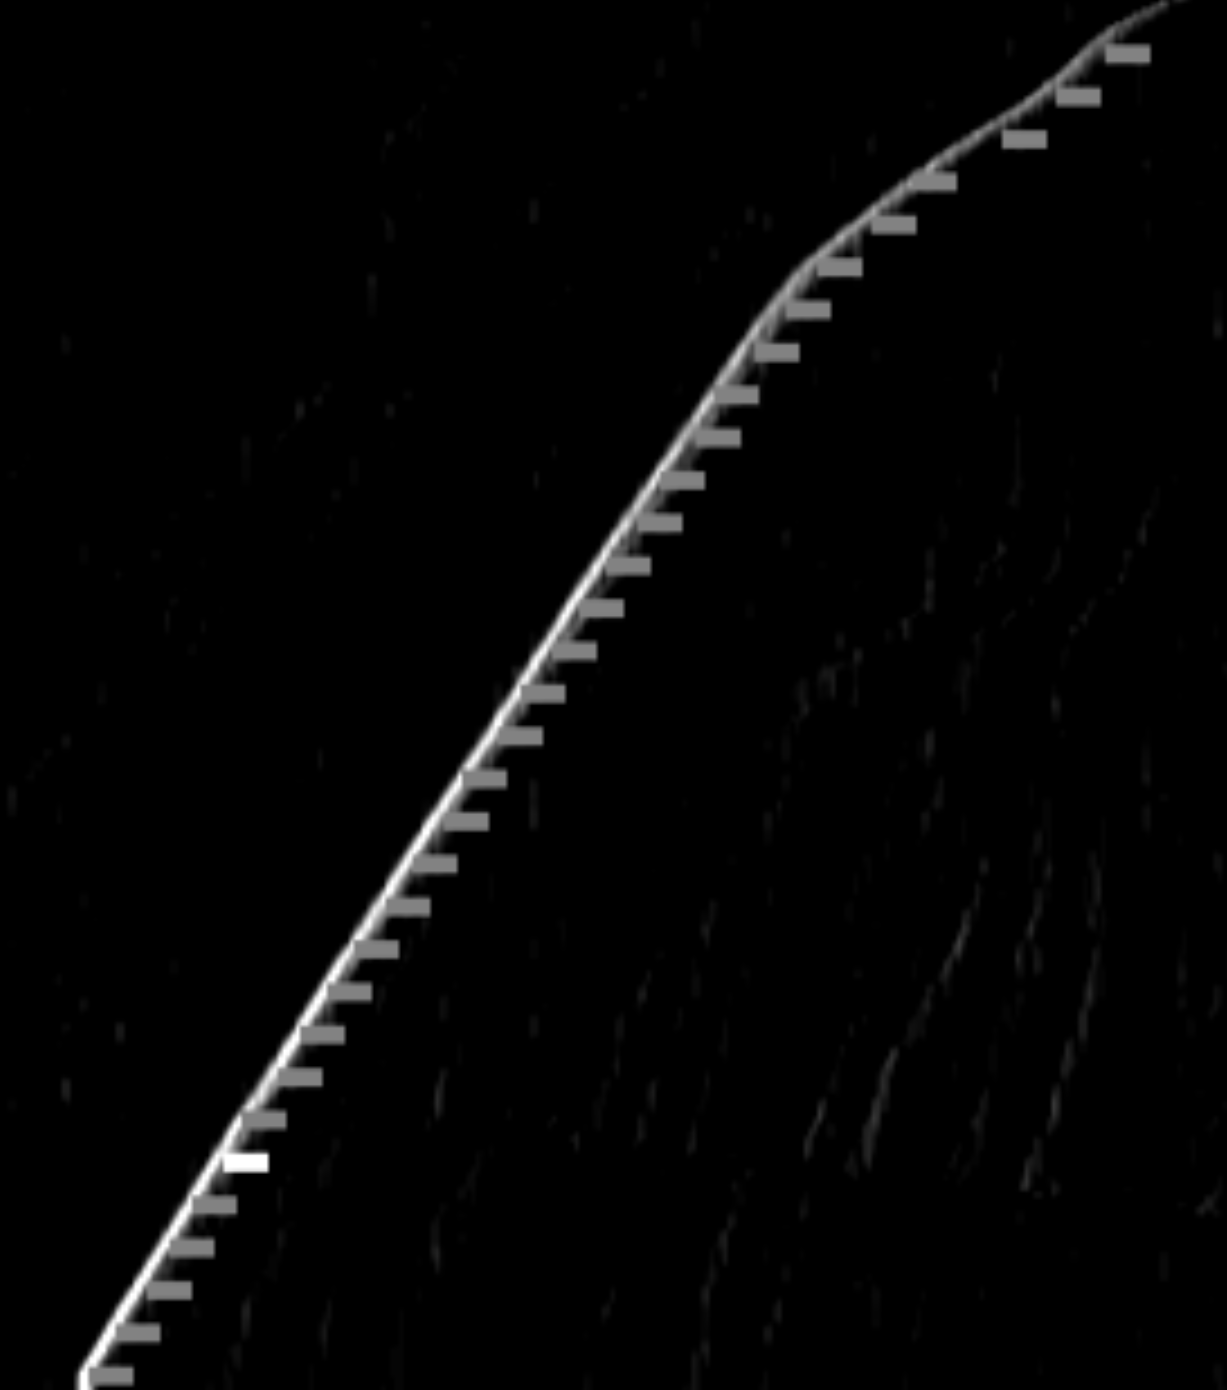
\includegraphics[width=\textwidth,height=0.2\textheight]{visionpipeline/straightoffsetleft.png}
                 \caption{Off Straight}
                 \label{fig:straight} 
              \end{subfigure}
              \hfill
              \begin{subfigure}[b]{0.32\textwidth}
                 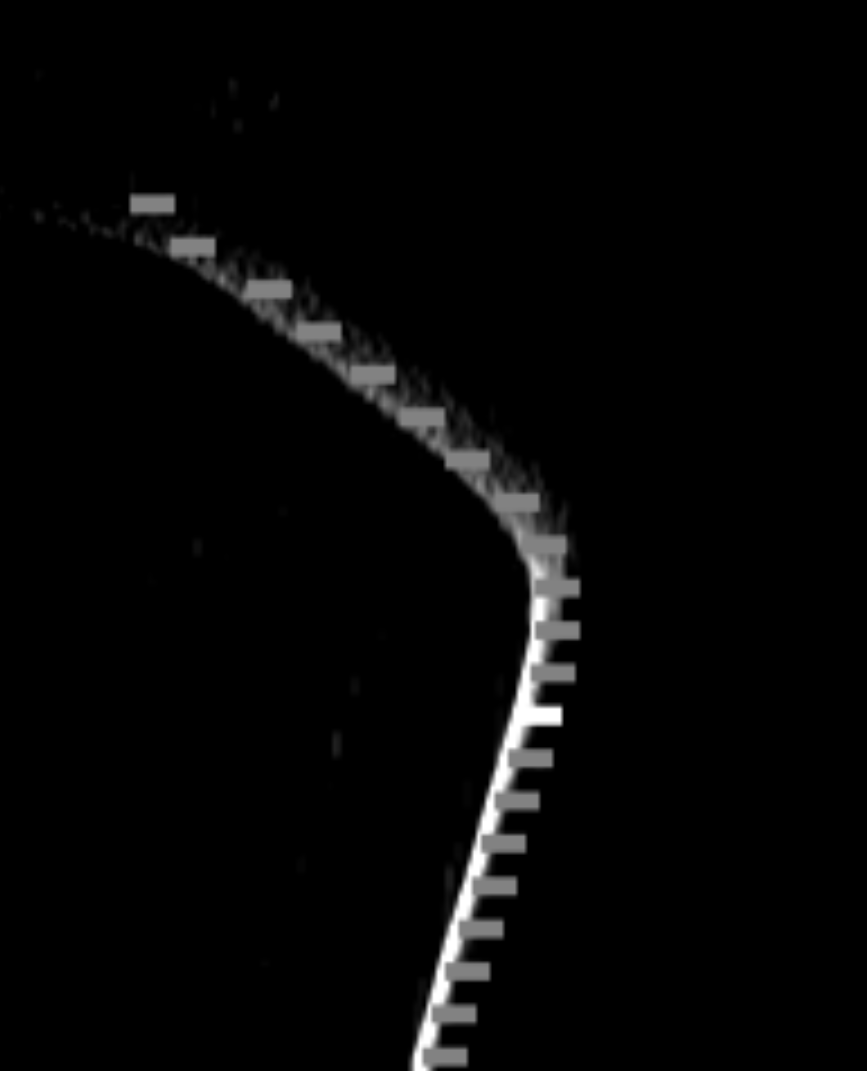
\includegraphics[width=\textwidth,height=0.2\textheight]{visionpipeline/apprachLeft.png}
                 \caption{Exit Chicane}
                 \label{fig:exitChicane}
              \end{subfigure}
              \caption{Path Waypoints}
              \label{fig:PathWayPoints}
           \end{figure}


        \begin{figure}[H]
            \centering
            \includegraphics[width=0.32\textwidth]{Diagrams/PurePersuit.pdf}
            \caption{Local Waypoint Following}
            \label{fig:PurePersuit}
        \end{figure}

        
        \pagebreak{}
        \subsection{Racing Algorithms}
            \subsubsection{Lateral Control}

            A bang-bang-type steering controller is used to obtain a baseline track performance. 
            This is a reactive controller which uses the cross track error, obtained via a topological peak tracker as described in section 6.2.
            In this case, the velocity target of the robot is set to some constant value. 
            The virtual sensor is applied to a small section of the bottom of the image frame, representing points on the track that are closest to the robot. 
            This manages to navigate the track without losing it on straights and gentle curves, however, it suffers on
            sharp sequences of curves, and chicanes, where the track in the observed section is lost or degraded. In this case, by rolling off the last known position 
            of the track towards the center of the image at each frame sample, and setting the velocity target to zero when no line is detected,
            the robot can navigate the track past the chicane. This control method is not robust or reliable and few trials can be performed where 
            the robot does not lose track and is forced to come to a stop.
            Despite the limitations in path-following accuracy, this simple method is capable of completing laps of the track at a
            low speed, \( v_{\text{max}} \ll 0.3 \, \text{m/s} \).
            This can be attributed to the implicit look ahead in the vision system, shown in Fig.\ref{fig:PurePersuit}, where the bottom of the image frame 
            captures the track some distance ahead of the robot and not exactly at its current position.
            
            
            \subsubsection{Adaptive Lookahead and Longitunal control}
            Constant parameter tuning is undesirable in a racing context as the robot must be able to adapt to the environment.
            Lookahead distance is one of such parameters that are often fixed or tuned experimentally,
            towards better racing performance, the failure cases of understeering on curves and oversteering on straights 
            are improved in 2 manners. The linear velocity of the robot is set to be inversely proportional to the number of waypoints found vision system,
            as this represents how much track there is ahead of the robot. This implicitly slows the robot down as it approaches a curve, 
            and handles adverse environmental conditions such as occlusions in the track automatically predictably, and safely. 
            It allows it to accelerate on a straights. By entering the cures at a lower speed, the robot no longer loses the track from its frame. 

            The chicane now poses a different challenge, as the robot must enter it slowly but it is desirable to accelerate out of it.
            Considering that upon entering the chicane, the longitudinal controller slows the robot down, so more of the track is visible, 
            hence to accelerate out of the curve the lookahead distance is increased inversely proportional to the number of waypoints. 
            This approach is counterintuitive as commonly, on straights, the looked distance is increased 
            and decreased on curves, however in the case of the TWSB robot, when the lookahead distance is too small the dead zone
            in the vision system causes the track to leave the image frame on sharp curves such at the apex of
            the chicane. By increasing the lookahead distance robot takes shallower turns, notably on the hairpin section of the track, enabling it to 
            increase its speed as the robot obtains a waypoint that is past the apex of the chicane allowing it to accelerate out 
            of the curve. This late apex racing strategy is commonly used by human racing divers \cite{kegelman2017insights}.
        
    \pagebreak{}


  %%%%%%%%%%%%%%%%%% SECTION 4 %%%%%%%%%%%%%%%%%%
  \section{Results and discussion} % edit section heading as appropriate
    \subsection{Balance Performance}

    A set of experiments are performed on the TWSB to evaluate the suitability of the controller designed in section 5 for the task of racing. 
    Data is collected at 100Hz and timestamped to ns resolution using the Raspberry Pi's internal clock. 

    The TWSB is righted from rest to a vertical position on a flat surface and the controller is activated. 

    \begin{figure}[H]
        \centering
        \includegraphics[width=0.7\textwidth]{Graphs/Static Balancing.pdf}
        \caption{Balance Performance}
        \label{fig:BalancePerformance}
    \end{figure}

    Fig.\ref{BalancePerformance} shows the 
    distribution pitch angle and x position as measured by the robot's sensors. 
    This experiment addresses the static balancing problem of the TWSB system, it was run continuously for 95 seconds,
    after which it was manually stopped. The results demonstrate that the robot maintains its position within ±1 mm 
    while regulating its pitch angle within ±1° of the vertical. The pitch distribution exhibits a sharp mode centered
    at approximately $-0.3\deg$, indicating a consistent, small offset from the theoretical upright equilibrium. 
    In contrast, the X position distribution is broader, with a relatively uniform frequency across the range. 
    This reflects low-amplitude, periodic oscillations in wheel position, which are intrinsic to the balancing process. 
    These oscillations result from the control effort required to counteract destabilizing torques and maintain upright stability. 
    Given that the 1 mm deviation represents less than $0.5\%$ of the wheel circumference.
    it can be concluded that the robot effectively maintains a static balance with negligible positional drift.
    \begin{figure}[H]
        \centering
        \includegraphics[width=0.7\textwidth]{Graphs/Disturbance Rejection.pdf}
        \caption{Disturbance Rejection}
        \label{fig:DisturbanceRejection}
    \end{figure}

    In the experiment shown in Fig.\ref{fig:DisturbanceRejection}, the robot is subjected to a series of external disturbances. 
    Rough terrain, including small household objects such as pens, coins, and other irregular items, is placed in its path. 
    Additionally, large impulsive forces are applied manually at approximately sample times $k = 800$ and $k = 3200$. 
    These disturbances displace the robot from its equilibrium, prompting it to regain balance by accelerating forward.
    Interestingly, even though the $x$ position is not explicitly regulated by the control system, 
    the TWSB robot gradually returns to its original position. As the robot traverses the small obstacles during this recovery, 
    minor oscillations are observed in the $x$ position signal, superimposed on the decaying trend back to zero.
    The pitch angle also responds to the disturbances, exhibiting transient overshoot relative to the 
    target angle  $\theta_{\text{trgt}}$. These results confirm the robot's ability to reject both terrain-induced 
    and impulsive external disturbances, while maintaining dynamic stability.

    \subsection{Velocity Tracking}

    Before testing the robot in a race track environment it must be verified that it can track velocity setpoints, accelerate, and most 
    importantly decelerate whilst maintaining balance. 
    \begin{figure}[H]
        \centering
        \includegraphics[width=0.7\textwidth]{Graphs/Velocity_Tracking.pdf}
        \caption{Velocity Tracking}
        \label{fig:VelocityTracking}
    \end{figure}

    In the experiment shown in Fig.\ref{fig:VelocityTracking}, the robot is commanded via a series of 
    ramp step functions to accelerate and decelerate at a constant rate. These aim to replicate the kinds of reference velocity profiles 
    the robot will have to perform if it is to achieve good lap times.
    The TWSB exhibits some minor lag in response tho the reference velocity, there is also some overshoot, which is 
    more significant when large decelerations are commanded. This can be attributed to the non-minimum phase of the system, 
    where the robot must first accelerate before it can decelerate, supplementing the velocity control with an acceleration 
    profile is a possible solution to this problem. Again, it can be seen that throughout this experiment the linear displacement 
    is driven to its 0 position when no velocity is commanded, even under large internal forces, this is a positive indication that the robot is able
    to perform well at its handling limits. In this experiment velocities were commanded up to 2 m/s, as above this the motors enter saturation 
    if operated continuously.

    \subsection{Path Following}
    The TWSB robot is tested on the track shown in Fig.\ref{fig:TestTrack}. Fiducial Markers are placed at the start position of the track and on the robot itself. 
    These are used by a top-down camera fixed to the ceiling, to track the position of the robot across many laps. The camera captures video at 30Hz in 1920x1080 resolution.
    The OpenCV library is used to track the April Tag on the robot, however, due to motion blur at high speeds it is unsuccessful in tracking the robot at all times, and 
    suffers especially on the straight section of the track where the robot is at its maximum velocity. Nevertheless, the obtained points are included in this analysis 
    as they provide a good indication path path-tracking performances, especially on the corners and other slow sections of the track. It also serves to demonstrate the discrepancies 
    between the real world, global localization, and the significant drift in position in the robot's inertial odometry. 

    A total of 80 Laps of the track were performed and recorded recorded several trials, these all used the same parameters for the controller but different limits on maximum velocities. 
    At each trial, the robot was reset to the start position and completed numerous laps of the track in a row. There was no human intervention in the control of the robot,
    and the separate trials were implemented as necessary for data collection.  The position of the tracker as sampled by the top-down fiducial tracker within its camera frame is 
    shown in Fig.\ref{fig:TrajTrack}. The track is obtained by common image processing contour extraction techniques.

    \begin{figure}[H]
        \centering
        \includegraphics[width=0.7\textwidth]{Graphs/Path Following.pdf}
        \caption{Top Down Fiducial Tracker}
        \label{fig:TrajTrack}
    \end{figure} 

    Here it can be seen that the robot is generally able to navigate the track. There are some cases where the position diverges from the rest 
    of the laps, notably about the first apex of the chicane, where occasionally there is some overshoot in position. The TWSB is still able to regain the track 
    and complete the lap in these cases. Further discussion of this is provided in section 7.4.
    As alluded to in the design of the waypoint tracking algorithm, adaptive changes to the lookahead distance, as denoted by the white marker in 
    Fig.\ref{fig:PathWayPoints}, causes the TWSB slightly understeers on entering the chicane and exiting the hairpin section of the track. 

    \subsection{Race Performance}

    The TWSB robot can consistently complete laps of the track. The figures below show the global position of the robot 
    as obtained by its odometry model, these are from the same trials as the fiducial tracking data. The discrepancy in the shape of the mapped track, and thus the 
    position accuracy of the robot is expected and is attributed to drift in odometry. Interestingly the odometry maps have a similar shape and begin diverging at sharp 
    curves, possibly due to the feathering of the linear and angular velocity increasing quantization errors at low speeds. Nevertheless, since the fiducial marker  
    is unable to obtain the global velocity profile of the laps, these figures provide an appropriate visualization for the discussion of the racing algorithm and strategy. 
    The robot travels clockwise around the track, and the start position is marked with a blue dot. The increase in maximum velocity of the TWSB between 
    Fig.\ref{fig:Slow Lap} and Fig.\ref{fig:Fast Lap} can be seen by the increase in track length where the robot exerts its maximum velocity, this is especially notable in the curves 
    where due to the faster velocity the robot can accelerate and decelerate in between corners, as opposed to a smooth constant velocity as seen in the slow lap. 
    At the chicane, the fast lap slows almost to a halt since it enters it a a speed greater than the maximum velocity achieved in the slow lap. Exiting the chicane it also accelerates smoothly 
    until it reaches the next corner. This is different from the baseline controller which does not implement the adaptive lookahead distance method and so takes the next corner gradually
    by threading the throttle as can be seen by the sections of low velocity in Fig.\ref{fig:baseline}. 

    In Fig.\ref{fig:Fail Recovery} the robot is shown to be able to recover from losing the track. Upon exiting the hairpin, it overshoots as 
    it did not slow down in the section that Fig.\ref{fig:Fast Lap} did. This causes a sudden stop, and the robot is required to turn slowly until it rejoins the track. 
    A similar case happens on exiting the chicane, where the robot has entered it at close to maximum velocity, and the track is lost. Again the TWSB comes to a sharp stop and manages to recover the 
    track. Even through these failures, the lap time is still significantly faster than the baseline and slow test lap. This indicates that if a good recovery system is in place 
    the robot can be pushed to its limits safely.

    Attempts were made to increase the maximum velocity of the robot to 2 m/s in line with the experiments in section 7.2, however with an acceptation profile, the pitch angle would 
    tilt too far back during sections of such high velocity causing the track to be completely lost from the camera frame, this in turn slowed the robot down but it was unable to recover the track 
    estimate and reliably complete more than 10 continues laps. Possibly a larger section of a straight would allow the robot to accelerate to this speed and then regulate the pitch
    angle to maintain the track, however this was not tested in this report.
   
    \begin{figure} [H]
        \centering
        \begin{subfigure}[b]{0.48\textwidth}
            \includegraphics[width=\textwidth]{Graphs/Velocity Profile_33_1.pdf}
            \caption{Slow Lap}
            \label{fig:Slow Lap}
        \end{subfigure}
        \hfill
        \begin{subfigure}[b]{0.48\textwidth}
            \includegraphics[width=\textwidth]{Graphs/Velocity Profile_40_1.pdf}
            \caption{Fast Lap}
            \label{fig:Fast Lap}
        \end{subfigure}
        \caption{Best Laps}
    \end{figure}  

    \begin{figure} [H]
        \centering
        \begin{subfigure}[b]{0.48\textwidth}
            \includegraphics[width=\textwidth]{Graphs/Velocity Profile_42_1.pdf}
            \caption{Baseline Controller}
            \label{fig:baseline}
        \end{subfigure}
        \hfill
        \begin{subfigure}[b]{0.48\textwidth}
            \includegraphics[width=\textwidth]{Graphs/Velocity Profile_34_1.pdf}
            \caption{Recovery From Loosing Track}
            \label{fig:Fail Recovery}
        \end{subfigure}
    \end{figure}




  %%%%%%%%%%%%%%%%%% SECTION 5 %%%%%%%%%%%%%%%%%%
  \section{Conclusions and future work} 
  \subsection{Conclusions}
    The experiments demonstrate that the hierarchical PID control strategy implemented for the two-wheel self-balancing robot is 
    highly effective in addressing both static and dynamic balance requirements, as well as the demands of a racing environment.
    During static balance tests, the robot maintained its pitch angle within $\pm1^\circ$ of the vertical and exhibited positional 
    deviations confined to within $\pm1$~mm, demonstrating negligible drift.
    Such precision confirms the efficacy of the control system in countering intrinsic oscillations and maintaining stability even under minor disturbances.

    In dynamic scenarios, the robot proved its robustness by effectively rejecting external disturbances.
    When subjected to irregular terrain and impulsive forces, the system transiently overshot in both pitch and position but quickly recovered 
    and returned to the desired equilibrium. This behavior underscores the controller's ability to counteract sudden perturbations
    while preserving overall stability. Additionally, the velocity tracking experiments revealed that the robot can accurately follow acceleration and 
    deceleration commands representative of race conditions, despite experiencing minor lags and overshoots. 
    These transients, attributed to the non-minimum phase nature of the system, did not detract from the robot's overall dynamic performance as it successfully returned 
    to its neutral state when no velocity was commanded.

    The path-following tests, which relied on a ceiling-mounted camera and fiducial markers, further validated the system's navigation capabilities over multiple 
    laps on a test track. Although high-speed motion induced occasional tracking inaccuracies due to motion blur, the adaptive waypoint tracking algorithm was effective
    in adjusting lookahead distances and ensuring that the robot maintained a predominantly correct path. This was particularly evident in curved sections, 
    where the robot's capacity to navigate corners through controlled acceleration and deceleration yielded improved lap times compared to a baseline controller.

    Ultimately, the successful integration of the hierarchical control strategy, along with the clear separation of subsystems, has resulted in a platform that is 
    both robust and adaptable. The experimental evidence suggests that taking a design approach which abstracts layers of autonomy allows for a system, which combined with its subsystems
    exceeds the performance requirements for a high-speed, agile two-wheel self-balancing robot. The system's ability to maintain balance, track desired velocities, 
    and recover from deviations highlights its potential for application in competitive environments, while also providing valuable learning and educational insights 
    for future enhancements in sensor fusion control and navigation strategies.
    \subsection{Future work}

    This project has successfully demonstrated the feasibility the a two-wheel self balancing robot designed in racing a a track at its limits of handling. 
    However, several areas for future work could enhance the performance and capabilities of the system. Firstly the system is currently reliant 
    on local odometry, and the top down camera fiducial tracker is inadequate for high-speed capture due to motion blur, as such a preliminary area of research 
    should be in obtaining, validating or designing a system which can accurately track the robot in an indoor environment in real-time to obtain accurate and reliable positional 
    data, this could be achieved using a combination of multiple cameras, Ultra Wideband position sensors or directly embedded a Lidar sensor on the robot. Once localization is achieved 
    the platform improvements to the local navigation can be made and verified such as obstacle avoidance, and global trajectory optimization can be made for achieving higher laps speeds. 
    Whilst an LQR might provide some design assurances, it is believed that larger performance gains could be achieved through developing a data driven or 
    learned model of the racing dynamics of the platform. Improvements can also be made to the mission algorithms, which currently only consumes $10\%$ of the Raspberry Pi's CPU time, 
    and so more data can be processed such as implementing optical flow for dynamical projecting the bird's eye view of the track.


  %%%%%%%%%%%%%%%%%% REFERENCES %%%%%%%%%%%%%%%%%%
    \printbibliography
  %%%%%%%%%%%%%%%%%% APPENDICES %%%%%%%%%%%%%%%%%%
  \begin{uomappendix} 
      \section{Code}
      The repository for this project can be found at 
      https://github.com/Wrodders/dBot
      \section{Risk assessment}
    \includegraphics[angle=90, width = 0.5\textheight]{Graphs/Risk Register Template.pdf}
    \section{Project plan}
    \includegraphics[angle=90, width = 0.5\textheight]{Project Plan.pdf}
    \section{Continued Professional Development}
    \includegraphics[angle=90, width = 0.5\textheight]{CPD.pdf}
      
  \end{uomappendix}


  
  %%%%%%%%%%%%%%%%%% END MATTER %%%%%%%%%%%%%%%%%%
  \end{document}